\documentclass{ieeeaccess}
\usepackage{cite}
\usepackage{amsmath,amssymb,amsfonts}
\usepackage{graphicx}
\usepackage{textcomp}
\usepackage{bm}
\usepackage{array}
\usepackage{multirow}
\usepackage{booktabs}
\usepackage{float}
\usepackage[section]{placeins}
\usepackage{url}

\makeatletter
\AtBeginDocument{\DeclareMathVersion{bold}
\SetSymbolFont{operators}{bold}{T1}{times}{b}{n}
\SetSymbolFont{NewLetters}{bold}{T1}{times}{b}{it}
\SetMathAlphabet{\mathrm}{bold}{T1}{times}{b}{n}
\SetMathAlphabet{\mathit}{bold}{T1}{times}{b}{it}
\SetMathAlphabet{\mathbf}{bold}{T1}{times}{b}{n}
\SetMathAlphabet{\mathtt}{bold}{OT1}{pcr}{b}{n}
\SetSymbolFont{symbols}{bold}{OMS}{cmsy}{b}{n}
\renewcommand\boldmath{\@nomath\boldmath\mathversion{bold}}}
\makeatother

\newcolumntype{+}{!{\vrule width 2pt}}
\newlength\savedwidth
\newcommand\thickcline[1]{%
  \noalign{\global\savedwidth\arrayrulewidth\global\arrayrulewidth 2pt}%
  \cline{#1}%
  \noalign{\vskip\arrayrulewidth}%
  \noalign{\global\arrayrulewidth\savedwidth}%
}
\newcommand\thickhline{\noalign{\global\savedwidth\arrayrulewidth\global\arrayrulewidth 2pt}%
\hline
\noalign{\global\arrayrulewidth\savedwidth}}

\renewcommand{\labelenumi}{(\arabic{enumi})}
\begin{document}
\history{}
\doi{}

\title{When Agreement Fails: Visual Anchoring and Multimodal Pseudo-Label Reliability in Classroom Behavior Recognition}

\author{\uppercase{Yan Ma}\authorrefmark{1}\authorrefmark{3} and \uppercase{Lizhuo Zhang}\authorrefmark{2}}

\address[1]{School of Education, Hunan Agricultural University, Changsha, China}
\address[2]{School of Information and Intelligent Science and Technology, Hunan Agricultural University, Changsha, China}
\address[3]{School of Foreign Studies, Changsha University of Science and Technology, Changsha, China}
\tfootnote{This work was supported by the Education Department of Hunan Province under Grant HNJG-2022-0608.}

\markboth
{Y. Ma and L. Zhang: When Agreement Fails}
{Y. Ma and L. Zhang: When Agreement Fails}

\corresp{Corresponding author: Lizhuo Zhang (e-mail: zhanglizhuo@hunau.edu.cn).}

\begin{abstract}
Dual-model agreement is widely used as a pseudo-label reliability
heuristic for multimodal large language models (MLLMs), but whether
agreement-filtered labels improve downstream fine-tuning in fine-grained
classroom behavior recognition remains uncertain.
This study presents a reproducible reliability-audit protocol that
evaluates agreement filtering under a single-frame protocol on three SCB
classroom behavior sub-datasets (BowTurnHead, HandriseReadWrite,
TeacherBehavior), linking bounding-box-level MLLM annotation quality
measurement, four filtering strategies, repeated-seed CLIP fine-tuning
(linear probe and LoRA), retention-ratio diagnostics, selective-routing
analysis, and an eleven-model cross-model robustness check spanning
seven model families (Qwen2, Qwen2.5, Qwen3.5, Qwen3.6, LLaVA, Gemma3,
and Gemma4) across 7B--35B parameter scales.

Three main findings emerge. First, agreement filtering is not a portable
denoising rule: on BowTurnHead, agreement-retained linear probing falls
to $15.53\% \pm 1.00\%$ while unfiltered pseudo-labels reach
$88.02\% \pm 0.12\%$, and retention-ratio controls confirm that this
collapse reflects class-composition shift and a label-quality ceiling
rather than sample count alone. Second, the operative constraint is
visual anchoring---the degree to which a category can be recovered from a
single frame without discourse context. Categories with low zero-shot
CLIP accuracy (e.g., \textit{guide}, \textit{answer}) systematically fail
across all tested MLLMs; newer-generation models (Qwen3.5-27B,
Gemma4-31B) substantially improve on \textit{guide} (53\% and 83\%
respectively) while \textit{answer} remains below 23\% universally,
identifying a task-level single-frame observability boundary. Third, a quality-threshold
experiment with Qwen3.5-27B pseudo-labels (annotation accuracy 50.3\%
vs.\ Qwen2-VL-7B's 41.2\%) locates the critical annotation accuracy range
between 41\% and 50\% at which pseudo-label fine-tuning crosses the
zero-shot baseline ($55.29\%$ vs.\ $53.43\%$). Together, these findings
show that downstream utility is gated by per-class visual anchoring and
annotation quality thresholds, which provide a task-internal screening
signal for deciding when MLLM pseudo-labels are likely to provide useful
supervision in classroom behavior recognition.
\end{abstract}

\begin{keywords}
classroom behavior recognition, multimodal large language models, pseudo-label filtering, visual anchoring
\end{keywords}

\titlepgskip=-15pt

\maketitle

%=================================================================
% 1. Introduction
%=================================================================
\section{Introduction}
\label{sec:intro}

\PARstart{A}{utomatic} recognition of classroom behaviors---teacher instructional
actions, student engagement postures, and off-task micro-movements---is
a prerequisite for scalable educational quality assessment and
intelligent classroom analytics~\cite{brophy2000teaching,anderson2004classroom}.
Supervised deep learning models have demonstrated strong recognition
performance on this task~\cite{li2022classroom_transformer,zhang2020classroom_cnn},
but they require large quantities of labeled images that are
labor-intensive to collect: a trained annotator must watch each video
clip, identify every person in the frame, draw bounding boxes, and
assign the correct activity label, often under ambiguous multi-label
conditions.
This annotation bottleneck severely limits the scale and diversity of
available classroom datasets, and motivates the search for
lower-cost labeling alternatives.

Multimodal large language models~(MLLMs) such as
Qwen~\cite{bai2023qwen} and LLaVA~\cite{liu2023llava}
have recently demonstrated impressive visual understanding across a
wide range of recognition tasks.
Given an image and a list of candidate categories, an MLLM can produce
a category prediction without any task-specific training, making them
practical candidates for automatic annotation pipelines.
Several recent studies have explored LLM-assisted annotation in
text-heavy domains~\cite{gilardi2023chatgpt,he2023annollm}, and
the LATTECLIP framework~\cite{cao2025latteclip} has shown that
MLLM-synthesized text descriptions can drive unsupervised CLIP
fine-tuning in general visual domains.
However, whether MLLMs can serve as reliable annotators for
\emph{fine-grained, domain-specific} behaviors---particularly those
requiring interpretation of pedagogical intent rather than surface
visual features---has not been systematically studied.

Classroom activity recognition poses distinctive challenges that
make this question non-trivial.
Some behaviors have clear visual signatures: a teacher writing on a
blackboard produces a characteristic image that any vision model should
recognise.
Others are intent-dependent: the visual difference between a teacher
``answering a student's question'' and a teacher ``giving a lecture''
may be imperceptible from a single frame.
This makes it plausible that MLLM annotation quality varies
substantially across categories, and that a simple pipeline of
``annotate everything, then fine-tune'' may be undermined by a small
number of systematically mis-labelled classes.
This paper refers to that category-specific degree of visual
identifiability as \emph{visual anchoring}.
Formally, visual anchoring is defined as the degree to which a
category label can be recovered from a single cropped frame without
recourse to discourse context, temporal information, or speaker intent.
The concept is used here as a task-internal diagnostic framework, not
as an independent causal measure.
The operational proxy employed in this study---protocol-matched per-class
zero-shot CLIP accuracy---is therefore interpreted as a screening signal
within this evaluation setup rather than as a universal quantification
of anchoring.

The practical motivation for studying agreement filtering deserves
explicit statement.
When two independently queried MLLM annotators assign the same label
to a crop, the probability that both are correct is generally higher
than for a single annotator.
This intuition---drawn from multi-annotator agreement in
crowdsourcing~\cite{snow2008cheap} and consistency-based semi-supervised
learning~\cite{laine2016temporal}---has made dual-model agreement a widely
adopted proxy for pseudo-label reliability.
However, this heuristic assumes that annotator errors are independent,
which may not hold when both models share architectural biases or
when the image itself lacks the visual evidence needed for the task.
Understanding when this assumption fails, and what the downstream
consequences are, is the central empirical question of this study.

From an engineering perspective, the practical question is not whether
MLLMs can produce pseudo-labels at all, but when those labels are
reliable enough to improve downstream adaptation and when filtering
removes the very supervision the model needs.

Against this background, the study addresses one central question:
\emph{when can MLLM-generated pseudo-labels provide a reliable training
signal for classroom behavior recognition, and when does agreement
filtering make that signal worse rather than better?}

Answering that question is operationalised through four linked analysis
modules rather than a chronological phase narrative.
First, a protocol-matched zero-shot CLIP baseline establishes the
training-free reference point under the same bounding-box crop setting.
Second, MLLM annotation and validation measure category-level
annotation reliability and test whether the observed failure modes
depend on the original annotator pair.
Third, CLIP adaptation under label-source choices compares unfiltered
pseudo-labels, agreement-filtered pseudo-labels, and ground-truth
supervision across linear probing and LoRA.
Fourth, mechanism and strategy audits use retention controls,
anchor-aware selective routing, auxiliary filtering and self-training
baselines, and cross-model consistency checks to distinguish between
data-volume loss, sampling bias, category semantics,
training-strategy effects, and annotator dependence.

The main pseudo-label annotation pipeline uses two MLLMs
(Qwen2-VL-7B-Instruct and LLaVA-1.5-7B) to annotate cropped
bounding-box regions from three SCB sub-datasets covering 13 behavior
categories across more than 87{,}000 bounding boxes.
An eleven-model robustness analysis (expanded from five models in the original submission) is treated as a boundary
condition check, not as the paper's main claim.
The core answer comes from the downstream fine-tuning matrix,
while the additional diagnostics explain why that answer changes across
datasets and categories.

The contributions are fourfold, with the audit protocol as the main
technical object rather than any single routing heuristic.

\begin{enumerate}

  \item \textbf{A reproducible reliability-audit protocol for MLLM
  pseudo-labeling.}
  The protocol connects bbox-level annotation accuracy, repeated-seed
  downstream CLIP adaptation, retention-ratio controls,
  distribution-shift checks, auxiliary training-strategy baselines,
  anchor-proxy analysis, and cross-model robustness.

  \item \textbf{Pseudo-label usefulness is category-conditional rather
  than global.}
  Visual anchoring separates classes that MLLMs can label reliably
  from classes that remain structurally ambiguous under single-frame
  crops.

  \item \textbf{Agreement filtering is not a safe denoising default.}
  The diagnostic evidence shows that agreement-filtered subsets can be
  affected by data-volume loss, class-composition shift, and shared
  label error, even when retained-subset annotation accuracy appears to
  improve.

  \item \textbf{The boundary conditions are separated from a single
  annotator choice or optimisation path.}
  An oracle selective-routing diagnostic, targeted LoRA replications,
  auxiliary teacher--student and confidence-filtering baselines, and a
  eleven-model robustness check bound the claim and point to label quality
  and category semantics as the main constraints in the present setting.

\end{enumerate}


%=================================================================
% 2. Related Work
%=================================================================
\section{Related Work}
\label{sec:related}

\subsection{Classroom Activity Recognition}

Automated analysis of classroom teaching and learning behaviors has
been approached through video~\cite{whitehill2014automated},
audio~\cite{donnelly2017automatic}, and multimodal
sensing~\cite{dillenbourg2011classroom}.
CNN-based methods achieved early success on student engagement
detection~\cite{zhang2020classroom_cnn}, and transformer architectures
have more recently enabled richer spatiotemporal
modelling~\cite{li2022classroom_transformer}.
A persistent challenge across all these works is the scarcity of
labeled data: classroom recordings raise privacy concerns, annotation
requires domain expertise, and activity categories are often defined
by pedagogical intent that is not directly visible in individual
frames.
The analysis addresses this bottleneck by evaluating whether
MLLMs can substitute for human annotators, thereby reducing labeling
cost.

\subsection{Vision--Language Models and Zero-Shot Transfer}

CLIP~\cite{radford2021learning} established contrastive
image--text pretraining as a powerful paradigm for zero-shot visual
recognition, enabling classification by matching image embeddings to
natural language category descriptions.
Subsequent work has extended this framework through improved training
data~\cite{schuhmann2022laion5b,cherti2023reproducible}, alternative
loss functions~\cite{zhai2023sigmoid}, masked image
modeling~\cite{sun2023eva02}, and data filtering
networks~\cite{fang2023data}.
Domain-specific applications include medical
imaging~\cite{wang2022medclip}, remote sensing~\cite{liu2024remoteclip},
and action recognition~\cite{wang2021actionclip}.
Zero-shot CLIP performance is known to be sensitive to prompt
design~\cite{radford2021learning}, and methods such as
CoOp~\cite{zhou2022learning} and CoCoOp~\cite{zhou2022conditional}
learn soft prompt embeddings to adapt CLIP to target domains with
minimal supervision.
In the classroom domain, however, zero-shot CLIP performance across
multiple scene types and model variants remains understudied.

\subsection{LLM- and MLLM-Assisted Data Annotation}

Using language models to generate or refine training labels has
attracted growing interest.
Early work showed that GPT-3/4-class models can produce competitive NLP
annotations for tasks such as stance classification and named entity
recognition~\cite{gilardi2023chatgpt,he2023annollm}.
In the multimodal setting, Zhang et al.~\cite{zhang2024zero} benchmark
zero-shot MLLM annotation for facial expression images, finding large
variance across model families and expression categories---a pattern
that parallels the results reported here.
However, that study stops at annotation benchmarking; it does not test
downstream CLIP adaptation, compare filtering protocols, or analyse why
particular categories fail.
Most relevant here is LATTECLIP~\cite{cao2025latteclip}, which
uses MLLM-generated rich textual descriptions to fine-tune CLIP without
any human labels in a general visual setting; the authors note that
annotation quality is especially low for classes that are ``not
visually discriminative,'' foreshadowing the visual anchoring
finding.
Recent open-weight MLLM progress in 2024--2025 has also changed the
practical annotation landscape.
Model families such as LLaVA-NeXT, Qwen2.5-VL, and InternVL2 report
stronger general visual reasoning and instruction following
capabilities~\cite{liu2024llavanext,qwen2025technical,chen2024internvl2},
while broader multimodal benchmarks such as MMMU still show that
domain-specific reasoning remains uneven and task dependent~\cite{yue2024mmmu}.
This is directly relevant to pseudo-label pipelines because better
average MLLM capability does not automatically imply reliable category
coverage under constrained prompts and single-frame evidence.
The work differs from LATTECLIP in three ways: it operates in a
fine-grained domain-specific setting, uses bounding-box-level rather
than image-level annotations, and explicitly characterises the
relationship between per-category annotation accuracy and downstream
fine-tuning performance.
More broadly, the paper combines three threads that are usually
treated separately: MLLM-based automatic annotation, pseudo-label
filtering, and classroom behavior recognition.
To the best of current knowledge, no prior work has systematically evaluated MLLM
annotation reliability for classroom activity recognition or provided
per-category diagnostic evidence of annotation failure modes.

\subsection{Pseudo-Label Filtering Strategies}

Filtering noisy pseudo-labels is a standard component of
semi-supervised and weakly supervised learning
pipelines~\cite{sohn2020fixmatch,zhang2021flexmatch}.
Common strategies include confidence thresholding, consistency
regularization across augmentations, and ensemble
agreement~\cite{laine2016temporal}.
In the classic semi-supervised setting, however, consistency filtering
usually compares predictions from the same model under perturbation or
augmentation, whereas this work examines agreement between two
different MLLMs on the same crop.
That distinction matters because cross-model agreement can remove not
only noisy samples but also large, systematically informative regions
of the training distribution when the two annotators fail in different
ways.
The agreement-based filter used here---retaining samples where two independently
queried MLLMs assign the same label---is conceptually related to
multi-annotator agreement in crowdsourcing~\cite{snow2008cheap}, where
consensus labels are generally higher quality but fewer in number.
Another major family of pseudo-label filtering methods uses calibrated
confidence or uncertainty estimates instead of agreement alone.
That comparison is relevant here, but the executed annotation protocol
uses index-only prompting and does not expose a calibrated
scalar confidence signal; for that reason, the experiments test
only the screening cues actually produced by the annotation pipeline,
namely valid-output screening and cross-model agreement.
A key finding is that, in the observed retention regime
(20--67\% on the training splits), the data-volume cost and sampling
bias of agreement filtering can overwhelm any quality benefit, leading
to substantial over-fitting or negligible downstream gains.
In these experiments, this pattern directly contradicts the common
intuition that cross-model agreement automatically yields better
training data.
This complements findings in the NLP annotation literature showing that
LLM label quality does not monotonically improve with filtering
stringency when the underlying model systematically errs on certain
input types~\cite{he2023annollm}.
Related 2024 reliability-oriented evaluations in multimodal settings
similarly suggest that robust deployment requires explicit uncertainty
or error-structure checks before assuming that stricter filtering
improves supervision quality~\cite{zhang2024zero,yue2024mmmu}.
Taken together, the gap in prior work is not the absence of MLLM
annotation studies, pseudo-label filtering methods, or classroom
recognition benchmarks in isolation, but the lack of a single study
that tests these components jointly and explains when and why the
combined pipeline fails in a classroom-behavior setting.

\section{Datasets and Experimental Setup}
\label{sec:method}

\subsection{Pipeline Overview}

The experimental pipeline consists of three stages, each producing
fixed artifacts consumed by downstream analyses:
\begin{enumerate}
  \item \textbf{Annotation stage:} YOLO-detected bounding-box crops are
  annotated by two MLLMs (Qwen2-VL-7B-Instruct and LLaVA-1.5-7B) under an
  index-only zero-shot prompt. Each crop receives a predicted class index
  from each model. Validation-set annotations are used only for quality
  measurement; training-set annotations are exported as JSONL for
  downstream fine-tuning.
  \item \textbf{Filtering stage:} Four filtering strategies are compared:
  None (all Qwen predictions), Valid-Output-Qwen (Qwen outputs a valid
  index), Valid-Output-LLaVA (LLaVA outputs a valid index), and Agreement
  (Qwen and LLaVA assign the same index). Only the None and Agreement
  strategies produce training pseudo-label JSONL files for the downstream
  stage.
  \item \textbf{Fine-tuning stage:} CLIP ViT-L/14 is fine-tuned under
  three label sources (None pseudo-labels, Agreement pseudo-labels, GT)
  and two training modes (linear probe, LoRA) across three SCB
  sub-datasets, forming an $18$-condition main matrix plus three
  zero-shot baselines. Four diagnostic modules---selective routing,
  retention-ratio curves, strategy audits (confidence filtering,
  teacher--student self-training, cross-model consistency), and a
  eleven-model cross-model robustness check---read frozen artifacts from
  earlier stages to isolate specific mechanisms.
\end{enumerate}

\subsection{Datasets}
\label{sec:datasets}

All experiments use three sub-datasets from the publicly available
SCB (Smart Classroom Behavior) benchmark~\cite{scb_dataset}, which
provides bounding-box annotations for classroom activity images
captured in real Chinese K--12 classrooms.
The three sub-datasets cover complementary scene types and difficulty
levels, summarised in Table~\ref{tab:datasets}.

\begin{table}[!t]
\caption{Overview of the three SCB sub-datasets used in this study,
including per-class bounding-box counts.
Class imbalance interacts with agreement filtering and anchor-aware routing
(Sec.~\ref{sec:discussion}).}
\label{tab:datasets}
\centering
\resizebox{\columnwidth}{!}{%
\begin{tabular}{llrrr}
\toprule
\textbf{Sub-dataset} & \textbf{Class} & \textbf{Train BB} & \textbf{Val BB} & \textbf{Train/Val images} \\
\midrule
\multirow{2}{*}{BowTurnHead (2-class)} & bow-head & 4{,}422 & 540 & \multirow{2}{*}{1{,}905 / 505} \\
 & turn-head & 7{,}943 & 3{,}213 & \\
\midrule
\multirow{3}{*}{HandriseReadWrite (3-class)} & hand-raise & 10{,}538 & 2{,}915 & \multirow{3}{*}{5{,}193 / 1{,}671} \\
 & read & 17{,}539 & 6{,}539 & \\
 & write & 6{,}447 & 3{,}394 & \\
\midrule
\multirow{8}{*}{TeacherBehavior (8-class)} & guide & 1{,}155 & 449 & \multirow{8}{*}{8{,}984 / 3{,}240} \\
 & answer & 2{,}574 & 853 & \\
 & on-stage interaction & 528 & 149 & \\
 & blackboard-writing & 821 & 277 & \\
 & teacher & 8{,}490 & 3{,}228 & \\
 & stand & 13{,}932 & 4{,}967 & \\
 & screen & 5{,}025 & 1{,}959 & \\
 & blackboard & 7{,}847 & 3{,}445 & \\
\bottomrule
\end{tabular}
}
\end{table}

Class balance is uneven in all three sub-datasets.
BowTurnHead is skewed toward \textit{turn-head}; HandriseReadWrite is
dominated by \textit{read}; and TeacherBehavior is dominated by
\textit{stand}, \textit{teacher}, and \textit{blackboard}, while
\textit{on-stage interaction} and \textit{blackboard-writing} are rare.
These imbalances provide relevant context for interpreting agreement
retention bias and selective-routing behavior.

\textbf{BowTurnHead} contains images of students exhibiting two
micro-action classes: \textit{bow-head} and \textit{turn-head}.
The \textit{bow-head} class typically corresponds to a downward head
posture associated with distraction or phone use.
The binary nature of the task and the visually distinct postures make
this the easiest sub-dataset.

\textbf{HandriseReadWrite} contains three student behavior classes:
\textit{hand-raise}, \textit{read}, and \textit{write}.
These classes require observing upper-body posture and hand position,
introducing moderate visual ambiguity between reading and writing.

\textbf{TeacherBehavior} contains eight teacher activity classes:
guide, answer, on-stage interaction, blackboard-writing, teacher
(general presence), stand, screen, and
blackboard.
The large class count, overlapping visual appearances, and the
prevalence of intent-dependent categories (e.g., ``answer'' versus
``guide'' are visually nearly identical) make this the most
challenging sub-dataset.

Throughout the manuscript, class names follow the index order used in
the annotation prompt and evaluation protocol:
BowTurnHead = \{0: \textit{bow-head}, 1: \textit{turn-head}\};
HandriseReadWrite = \{0: \textit{hand-raise}, 1: \textit{read},
2: \textit{write}\};
TeacherBehavior = \{0: \textit{guide}, 1: \textit{answer},
2: \textit{on-stage interaction}, 3: \textit{blackboard-writing},
4: \textit{teacher}, 5: \textit{stand}, 6: \textit{screen},
7: \textit{blackboard}\}.

All annotations are provided in YOLO format (class index, normalised
centre coordinates, width, height).
Each bounding box defines a single activity instance; images may
contain multiple bounding boxes corresponding to different individuals
or simultaneous activities.

\subsection{Ethics and Data Governance}

This study is a secondary analysis of a previously released public
benchmark of classroom images and bounding-box annotations.
The authors did not recruit participants, collect new data, intervene
in classroom activities, or access metadata beyond the released image
and label files.
The analysis uses only the released benchmark files, reports aggregate
results, and does not reproduce identifiable classroom images.
Under this secondary-analysis design, additional institutional review
and informed consent were not required for the present study.
Ethical oversight for the original classroom data collection remains
with the SCB dataset creators and the institutions that approved its
release.
The present work relies on those original approvals and follows the
authors' institutional policy for secondary analysis of public child
image datasets: no re-identification attempts, no release of new
identifiable child images, and aggregate-only reporting.
All qualitative examples in the manuscript are privacy-preserving
pixelated crops generated for illustration, and the study does not
redistribute raw classroom images outside the public dataset release.

\subsection{MLLM Annotation Pipeline}
\label{sec:annotation}

\subsubsection{Bounding Box Cropping}

For each annotated bounding box, the corresponding image region is
cropped with a 5\% margin on each side to provide contextual
information around the target.
Crops smaller than $32 \times 32$ pixels after margin expansion are
discarded.
This yields 87{,}261 training crops and 31{,}928 validation crops
across the three sub-datasets.

\subsubsection{Models}

In the main pseudo-label annotation pipeline, two locally deployable
MLLMs serve as annotators:
\textbf{Qwen2-VL-7B-Instruct}~\cite{bai2023qwen} (hereafter Qwen)
and \textbf{LLaVA-1.5-7B}~\cite{liu2023llava} (hereafter LLaVA),
both running on dedicated GPUs to enable parallel annotation.
The study selects locally deployable 7B-scale models for three reasons:
reproducibility without API dependency, cost-free inference at scale,
and comparability between the two models under identical hardware
conditions.

\subsubsection{Prompt Design}

Both models receive a uniform zero-shot prompt listing the category
names with their indices, followed by the instruction to respond with
the index only:

\begin{quote}
\textit{You are a classroom behavior recognition expert.
Given one cropped classroom image, choose the single best matching
class. Reply with only the class index number. No explanation.
Classes: [0: class\_0, 1: class\_1, \ldots]. Answer with index only:}
\end{quote}

The same prompt serves all three sub-datasets; only the class list
changes.
No dataset-specific synonyms, textual definitions, or auxiliary class
descriptions are added beyond the class names shown in the prompt.
This index-only format standardises the output space across models and
reduces parsing ambiguity, but it does not measure uncertainty and may
force low-confidence decisions into a single discrete label.
For all executed annotation runs, decoding is deterministic
(\texttt{do\_sample=False}), and the response length is capped at
\texttt{max\_new\_tokens=8}.

Table~\ref{tab:index_mapping_audit} summarises the label-index order
used in the executed runs. The same dataset-specific class list is
passed to both MLLMs from a shared dataset configuration, and downstream
evaluation reuses the same order for label decoding. Valid model outputs are single in-range
integers such as ``0'', ``1'', or ``4''; any non-integer or out-of-range
string is recorded as invalid instead of coerced to a class label.

\begin{table}[!t]
\caption{Label-index order audit for the index-only prompt. The same
ordering is used for both MLLM annotation and downstream label decoding,
providing a direct consistency check against index-mapping errors.}
\label{tab:index_mapping_audit}
\centering
\resizebox{\columnwidth}{!}{%
\begin{tabular}{lp{10.6cm}}
\toprule
\textbf{Dataset} & \textbf{Index order used in prompt and evaluation} \\
\midrule
TeacherBehavior & 0: guide; 1: answer; 2: on-stage interaction; 3: blackboard-writing; 4: teacher; 5: stand; 6: screen; 7: blackboard \\
HandriseReadWrite & 0: hand-raise; 1: read; 2: write \\
BowTurnHead & 0: bow-head; 1: turn-head \\
\bottomrule
\end{tabular}
}
\end{table}

Fig~\ref{fig:pipeline} summarizes the full experimental pipeline,
from bbox cropping and MLLM annotation to pseudo-label filtering,
CLIP fine-tuning, and diagnostic interpretation.

\begin{figure}[!t]
\centering
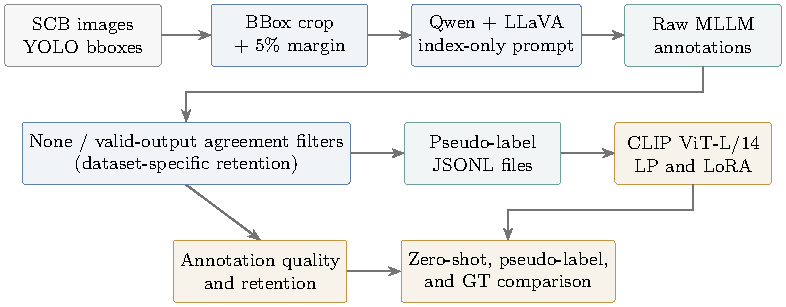
\includegraphics[width=0.98\linewidth]{fig_pipeline_access.pdf}
\caption{Experimental pipeline for MLLM-assisted classroom behavior annotation.
Bounding-box crops are annotated by two 7B-scale MLLMs, converted into
pseudo-label sets through filtering strategies, and used to fine-tune
CLIP with linear probing or LoRA. The same pipeline also yields
annotation-quality and retention diagnostics.}
\label{fig:pipeline}
\end{figure}

\subsubsection{Filtering Strategies}

For implementation audit purposes, the pipeline records four filtering
variants, but only two of them represent substantively different
selection rules under the executed protocol:

\begin{enumerate}
    \item \textbf{None (unfiltered):} All crops for which Qwen
    produces a valid index are retained.
    The pipeline uses the Qwen prediction as the pseudo-label.

    \item \textbf{Valid-Output-Qwen:} Only crops where Qwen outputs
    a valid in-range index are retained (identical to None in
    practice, as Qwen has a near-100\% valid-output rate).

    \item \textbf{Valid-Output-LLaVA:} Only crops where LLaVA outputs
    a valid index are retained.

    \item \textbf{Agreement:} Only crops where Qwen and LLaVA assign
    the same index are retained; crops with disagreement are excluded,
    and the shared index is used as the pseudo-label.
\end{enumerate}

Because the annotation prompt enforces an index-only response and does
not expose calibrated confidence scores, confidence thresholding is not
available as a distinct scalar filter in the executed runs.
In practice, Valid-Output-Qwen collapses to None and Valid-Output-LLaVA
differs only through valid-output screening, so the
downstream analysis focuses on None and Agreement as the two
informative representative strategies.
The goal of this comparison is not to optimise a confidence
threshold, but to test whether the readily available screening signals
produced by the executed annotation protocol---valid-output screening
and cross-model agreement---improve over unfiltered pseudo-labels under
the same prompt and crop setting.

\subsection{CLIP Fine-Tuning}
\label{sec:finetune}

\subsubsection{Backbone}

CLIP ViT-L/14 with OpenAI pretrained
weights~\cite{radford2021learning} serves as the visual backbone
throughout,
matching the model family used in prior zero-shot evaluation on these
datasets~\cite{scb_dataset}.
The implementation uses \texttt{open\_clip\_torch} version 2.32.0.
The image encoder produces 768-dimensional embeddings.

\subsubsection{Fine-Tuning Methods}

Two parameter-efficient fine-tuning strategies are compared:

\textbf{Linear Probe (LP):} The CLIP visual encoder is fully frozen.
A single linear classification head ($768 \to C$, where $C$ is the
number of classes) is trained on the pseudo-labeled crops using
cross-entropy loss.

\textbf{Low-Rank Adaptation (LoRA):} LoRA layers~\cite{hu2022lora}
with rank $r=8$ and scaling factor $\alpha=16$ are injected into the
two MLP layers (\texttt{mlp.c\_fc} and \texttt{mlp.c\_proj}) of all
transformer blocks in the visual encoder.
LoRA layers are injected only into the MLP projections, as replacing
the \texttt{MultiheadAttention} output projection in the \texttt{open\_clip}
implementation interfered with direct access to the underlying
\texttt{out\_proj.weight} and \texttt{out\_proj.bias} attributes.
This introduces 1.97M LoRA parameters while keeping the remaining
$\sim$303M CLIP parameters frozen.
The linear classification head is trained jointly with the LoRA
parameters.

\subsubsection{Training Details}

All models are trained for 20 epochs using AdamW optimiser
($\text{lr}=10^{-4}$, weight decay $= 0.01$) with cosine annealing
learning rate schedule.
The reported main-matrix and targeted-replication runs use batch size
128, distributed across two NVIDIA
A100-SXM4-40GB GPUs via \texttt{DataParallel}.
No gradient accumulation is used, so the effective optimisation batch
size equals the per-step global batch size specified in each run.
Best model selection is based on validation accuracy.
For the main downstream matrix, LP conditions are averaged over
repeated seeds (all datasets: five seeds, 43--47). A targeted LoRA replication over five seeds
(43--47) is reported for BowTurnHead and TeacherBehavior under None
and GT; the remaining LoRA values stay as protocol-matched single-run
evaluations (seed 42).
Retention-ratio and selective-routing diagnostics are reported as
fixed-seed runs (seed 42).
An overview of seed usage by module is provided in
Table~\ref{tab:seed_policy}.
Pseudo-label generation and CLIP fine-tuning remain split-isolated:
validation crops are used only for annotation evaluation and model
selection, whereas pseudo-label files consumed by CLIP fine-tuning are
generated exclusively from the training split.

\subsubsection{Experimental Conditions}

For each of the three sub-datasets and two fine-tuning methods,
the study evaluates three pseudo-label sources:

\begin{itemize}
    \item \textbf{None:} Unfiltered MLLM pseudo-labels (Qwen predictions).
    \item \textbf{Agreement:} Agreement-filtered pseudo-labels.
    \item \textbf{GT:} Ground-truth human annotations (supervised reference).
\end{itemize}

This yields $3 \times 2 \times 3 = 18$ experimental conditions in total.
The zero-shot CLIP baseline (no fine-tuning,
prompt-engineered text embeddings) provides the primary practical
reference.
Prompt-adaptation methods such as CoOp and CoCoOp are not included as
direct baselines here because they require target-domain optimisation;
this comparison isolates the value of pseudo-label supervision
against a training-free reference and a ground-truth upper bound under
the same crop protocol.
The main-result zero-shot values (Table~\ref{tab:main_results}) are
obtained under the same bbox-crop validation protocol using the
canonical zero-shot evaluation setting.
Per-class prompt-ensemble outputs from the same
evaluation pipeline are used separately in the anchor-proxy
analysis and the selective-routing experiment.

\begin{table}[!t]
\caption{Seed policy by analysis module.
Main-matrix LP uses repeated-seed evaluation; targeted LoRA
replication is reported for BowTurnHead and TeacherBehavior under None
and GT; auxiliary diagnostics and the remaining LoRA reference cells
remain protocol-matched single-run/fixed-seed analyses.}
\label{tab:seed_policy}
\centering
\resizebox{\columnwidth}{!}{%
\begin{tabular}{>{\raggedright\arraybackslash}p{4.0cm}>{\raggedright\arraybackslash}p{4.8cm}>{\raggedright\arraybackslash}p{3.0cm}}
\toprule
\textbf{Module} & \textbf{Protocol scope} & \textbf{Seed policy} \\
\midrule
Main downstream matrix (LP) & 3 datasets $\times$ 3 label sources & 5 seeds (43--47) \\
Targeted LoRA replication & BowTurnHead + TeacherBehavior; None/GT & 5 seeds (43--47) \\
Main downstream matrix (remaining LoRA) & HandriseReadWrite + agreement conditions & single run (42) \\
Retention-ratio curves & 3 datasets, LP diagnostics & fixed seed (42) \\
Selective routing (Scheme B) & TeacherBehavior oracle diagnostic & fixed seed (42) \\
Auxiliary filtering/self-training baselines & 3 datasets, LP diagnostics & 5 seeds (43--47) \\
Cross-model annotation and consistency check & 5 MLLMs annotation quality & deterministic eval protocol \\
\bottomrule
\end{tabular}
}
\end{table}

\subsection{Integrated Diagnostic Analyses}
\label{sec:additional_experiments}

Beyond the main annotation-quality and downstream fine-tuning
comparisons, the study design includes linked diagnostic analyses.
Each addresses a different decision point in the pseudo-labeling
workflow: whether categories are visually grounded enough for automatic
annotation, whether agreement filtering fails because of retention loss
or sampling bias, whether category-aware routing can serve as an
upper-bound diagnostic on the hardest taxonomy, whether simple
confidence-filtering or self-training alternatives change the
downstream interpretation, and whether the main annotation patterns
remain stable under model substitution.
Together, these analyses are intended to explain the main findings,
not to replace repeated-seed downstream validation.

\subsubsection{Selective Annotation (Scheme~B)}

To validate the diagnostic utility of visual anchoring as an annotation
routing criterion, the study runs a selective annotation experiment on
TeacherBehavior.
The four high-anchor categories---\textit{blackboard-writing},
\textit{teacher}, \textit{screen}, and \textit{blackboard}---are
trained using unfiltered pseudo-labels (None strategy) with a linear
probe classification head restricted to those four classes.
This selective routing is evaluated only as an oracle upper-bound
diagnostic, not as a directly deployable pipeline.
The four low-anchor categories---\textit{guide}, \textit{answer},
\textit{on-stage interaction}, and \textit{stand}---are not included
in fine-tuning; at inference time, these categories are handled by the
frozen zero-shot CLIP classifier built with a prompt ensemble.
During offline evaluation, the final prediction for each validation
crop selects the fine-tuned head for high-anchor inputs and the
zero-shot classifier for low-anchor inputs using the ground-truth
category only as an oracle routing variable.
The resulting overall 8-class accuracy should therefore be interpreted
strictly as an upper-bound diagnostic for category-aware routing, not
as a directly deployable inference pipeline.
A deployable variant would need a separate routing predictor derived
from observable cues or proxy scores instead of ground-truth labels.

Pilot implementation tests with LoRA showed rapid overfitting and
severe degradation of the low-anchor zero-shot branch, because LoRA
modifies the shared visual encoder used by both branches.
For this reason, Scheme~B reporting focuses on linear probing.

\subsubsection{Retention-Ratio Curve}

To characterise the relationship between training data volume and
downstream performance more precisely than the two-endpoint comparison
afforded by the None versus Agreement conditions, the study evaluates
intermediate retention ratios of 25\%, 50\%, and 75\% on BowTurnHead
and HandriseReadWrite.
For each ratio, a random subset of the corresponding size is drawn
from the unfiltered pseudo-label training set (fixed seed 42), and
a linear probe is trained for 20 epochs under identical hyper-parameters.
The resulting five-point curves (25\%, 50\%, 75\%, 100\% from step3,
and the Agreement endpoint) provide a finer-grained view than a simple
two-endpoint comparison. These retention-ratio diagnostics intentionally
remain fixed-seed comparisons so that data-volume effects can be read
against a single controlled subset draw; the main LP results in
Table~\ref{tab:main_results} instead report repeated-seed averages
(all datasets: five seeds, 43--47).

\subsubsection{Auxiliary Filtering and Teacher--Student Baselines}

Two auxiliary training-strategy baselines test whether simple
alternatives to the main pseudo-label protocol change the downstream
interpretation. The confidence-filtering baseline starts from the
unfiltered Qwen pseudo-label training set. Each training crop is encoded
with CLIP ViT-L/14, the same prompt-ensemble zero-shot classifier is
constructed, and the CLIP probability assigned to the Qwen pseudo-label
is used as a confidence score. Linear probes are then trained on the
retained samples for thresholds $\{0.3,0.5,0.6,0.7,0.8,0.9\}$ across
seeds 43--47. Because the MLLM prompt uses index-only outputs, this
score is a CLIP-assisted confidence proxy, not calibrated MLLM logit
confidence.

The teacher--student baseline evaluates a label-scarce self-training
alternative under the same CLIP feature protocol. For each seed, a
linear-probe teacher is trained on a stratified 10\% labeled subset of
the training split. The teacher then assigns pseudo-labels to the
remaining training crops, and a student linear probe is trained on those
teacher labels together with the labeled training subset. Validation
labels are not used as training labels; they are used only for model
selection and evaluation under the same validation protocol as the main
LP experiments. This baseline is a label-scarce reference for
semi-supervised training under limited human annotation, not a label-free
alternative to the MLLM pseudo-labeling pipeline.

\subsubsection{Cross-Model Robustness Boundary Check}

To test whether the main annotation findings depend strongly on the
original two-model main pipeline (Qwen2-VL-7B and LLaVA-1.5-7B), the
revised study includes an expanded cross-model robustness check with eleven
open-weight MLLMs spanning seven model families (Qwen2, Qwen2.5, Qwen3.5,
Qwen3.6, LLaVA, Gemma3, and Gemma4), three architectural types (dense,
MoE, and 4-bit quantized), and parameter scales from 7B to 35B:
Qwen2-VL-7B-Instruct, LLaVA-1.5-7B, Qwen2.5-VL-7B-Instruct,
Qwen2.5-VL-32B-Instruct, Qwen3.5-27B, Qwen3.5-35B-A3B (MoE),
Qwen3.6-27B, Qwen3.6-35B-A3B (MoE, FP8), Gemma-3-27B-IT (4-bit),
Gemma4-26B-A4B-it (MoE), and Gemma4-31B-it.
All runs use the same bbox-crop protocol, index-only prompt, and
label decoding as the main annotation pipeline.
Validation annotations are collected for all three sub-datasets;
TeacherBehavior is additionally processed on the training split to
check whether the same category-level failure pattern persists outside
the validation set.
The cross-model analysis focuses on per-model pseudo-label accuracy and
on pairwise agreement-subset accuracy among model pairs, and the
expanded model set allows testing whether the observed failure patterns
generalise across model generations, architectures, and scales.
This robustness check strengthens external validity with
respect to annotator choice, but it does not by itself resolve the
within-protocol variance question created by the remaining
single-run downstream settings.

\subsubsection{Operational Proxy for Visual Anchoring}

To make visual anchoring operational here, the analysis
defines a category-level proxy score using protocol-matched per-class
zero-shot CLIP accuracy:
\[
\mathrm{AnchorProxy}(y)=\mathrm{Acc}^{\mathrm{ZS}}_{y}.
\]
Here, $\mathrm{Acc}^{\mathrm{ZS}}_{y}$ denotes the per-class accuracy of
zero-shot CLIP (prompt-ensemble setting) under the same bbox-crop
validation protocol used for all downstream experiments.
Higher values indicate that category $y$ is more visually anchored,
whereas lower values indicate stronger dependence on intent or context.
This proxy supports diagnostic interpretation and is not claimed as
a causal estimator or as an independent ground-truth measure of visual
anchoring.
Because the proxy is derived from another classifier's observed
performance, it should be interpreted as an operational screening cue
within this evaluation setup, not as an independent explanatory
measurement.
As a convergent diagnostic, the study also reports a class-level
cross-model consistency (CMC) score computed from the eleven MLLM
annotators. For each ground-truth category, CMC is the mean pairwise
agreement among model predictions on validation crops from that
category. CMC is independent of the CLIP zero-shot classifier used to
construct $\mathrm{AnchorProxy}$, but it is still treated as a
descriptive consistency signal, not as a causal measure of
anchoring.
In addition, because Scheme~B routes low-anchor classes through the
same zero-shot CLIP branch used to construct
$\mathrm{AnchorProxy}(y)$, these two signals are operationally
coupled here and should not be interpreted as independent
confirmatory evidence.

%=================================================================
% 4. Results
%=================================================================
\section{Results}
\label{sec:results}

Results are organised around the paper's central question, not around
the repository's execution order.
The section first establishes where MLLM pseudo-labels are reliable
enough to serve as plausible training signal, using annotation-quality
and per-category evidence.
It then tests whether those pseudo-labels actually help downstream
CLIP adaptation relative to zero-shot inference and the ground-truth
reference.
Finally, diagnostic and robustness analyses delimit why agreement
filtering fails and how strongly the conclusions depend on annotator
choice.

\subsection{MLLM Annotation Quality}
\label{sec:annot_quality}

Table~\ref{tab:annotation_quality} reports pseudo-label accuracy and
retention rates for the None and Agreement strategies on the
validation split of each sub-dataset.
Each retained bounding-box crop is treated as one evaluation instance,
so both accuracy and retention are defined at bbox level, not at
whole-image level.

\begin{table}[!t]
\caption{MLLM pseudo-label annotation accuracy and retention rate
on the validation split. ``Pseudo-label acc.'' = percentage of pseudo-labels
matching the ground-truth label for retained bbox crops. Under the None strategy,
``Retained'' is the number of crops with a valid Qwen index; Qwen
produces valid outputs for more than 99.9\% of validation crops.
These retention rates are computed on the validation split only;
training-set retention rates used later in the retention-ratio analysis
are reported separately in the text and figure.}
\label{tab:annotation_quality}
\centering
\resizebox{\columnwidth}{!}{%
\begin{tabular}{lccccc}
\toprule
\multirow{2}{*}{\textbf{Sub-dataset}} &
\multicolumn{2}{c}{\textbf{None (Qwen)}} &
\multicolumn{3}{c}{\textbf{Agreement (Qwen+LLaVA)}} \\
\cmidrule(lr){2-3}\cmidrule(lr){4-6}
 & \shortstack{Pseudo-label\\acc. (\%)} & Retained & \shortstack{Pseudo-label\\acc. (\%)} & Retained & Ret. rate (\%) \\
\midrule
BowTurnHead       & 82.55 & 3{,}753 & 41.76 & 613  & 16.3 \\
HandriseReadWrite & 70.60 & 12{,}843 & 73.97 & 7{,}122 & 55.4 \\
TeacherBehavior   & 41.21 & 15{,}327 & 47.57 & 10{,}167 & 66.3 \\
\bottomrule
\end{tabular}
}
\end{table}

Three observations follow.
First, annotation accuracy decreases monotonically with task
complexity: from 82.6\% for the binary BowTurnHead to 41.2\% for the
eight-class TeacherBehavior.
Second, Agreement filtering is not a uniformly reliable default: it improves
retained-subset accuracy on HandriseReadWrite and TeacherBehavior, but
substantially reduces both retention and accuracy on BowTurnHead.
Only 16.3\% of BowTurnHead validation crops survive the agreement
filter, and their accuracy falls from 82.55\% to 41.76\%.
Third, even after filtering, annotation accuracy remains well below the
ground-truth reference for HandriseReadWrite and TeacherBehavior.
To avoid ambiguity, the manuscript distinguishes these validation-set
retention rates (16.3\%, 55.4\%, and 66.3\%) from the training-set
retention rates used in downstream fine-tuning (20.0\%, 55.9\%, and
66.5\%).

Pairwise cross-model agreement follows the same pattern. Because both
models produce valid outputs for almost every validation crop, the
agreement rate is 16.33\% on BowTurnHead, 55.46\% on
HandriseReadWrite, and 66.33\% on TeacherBehavior, leaving
corresponding disagreement rates of 83.67\%, 44.54\%, and 33.67\%.
BowTurnHead is the clearest failure case: the two models disagree on
3{,}140 of 3{,}753 validation crops, so the agreement filter keeps only
a small and highly selective subset, not a uniformly cleaner one.

\begin{table}[!t]
\caption{BowTurnHead validation-set confusion counts for Qwen and
LLaVA. Rows denote ground-truth labels; columns denote model
predictions.}
\label{tab:bow_confusion}
\centering
\resizebox{\columnwidth}{!}{%
\begin{tabular}{lrrrr}
\toprule
\textbf{GT class} & \textbf{Qwen$\to$bow} & \textbf{Qwen$\to$turn} & \textbf{LLaVA$\to$bow} & \textbf{LLaVA$\to$turn} \\
\midrule
bow-head  & 237 & 303 & 534 & 6 \\
turn-head & 352 & 2{,}861 & 3{,}193 & 20 \\
\bottomrule
\end{tabular}
}
\end{table}

Table~\ref{tab:bow_confusion} clarifies why agreement filtering
collapses on BowTurnHead. Qwen predicts \textit{turn-head} on most
\textit{turn-head} crops, whereas LLaVA collapses almost the entire
\textit{turn-head} class into \textit{bow-head}. The dominant
disagreement pattern is ground-truth \textit{turn-head} with
Qwen = \textit{turn-head} and LLaVA = \textit{bow-head}
(2{,}842 crops), followed by ground-truth \textit{bow-head} with
Qwen = \textit{turn-head} and LLaVA = \textit{bow-head}
(297 crops). Within the 613 agreed crops, the models jointly predict
only 19 \textit{turn-head} instances correctly but jointly mislabel
351 \textit{turn-head} instances as \textit{bow-head}, so agreement
selects shared bias, not shared correctness.

\subsubsection{Per-Category Analysis of TeacherBehavior}

Table~\ref{tab:per_class} presents per-category annotation accuracy
under the Agreement strategy for TeacherBehavior, revealing a
clear bimodal distribution.

\begin{table}[!t]
\caption{Per-category MLLM annotation accuracy on TeacherBehavior
(Agreement strategy, validation split). Accuracy is reported to two
decimal places to match the other quantitative tables.}
\label{tab:per_class}
\centering
\begin{tabular}{lcc}
\toprule
\textbf{Category} & \textbf{Accuracy (\%)} & \textbf{n} \\
\midrule
blackboard-writing  & 98.61 & 216  \\
teacher             & 92.01 & 2{,}729 \\
screen              & 69.41 & 1{,}154 \\
blackboard          & 57.42 & 2{,}238 \\
\midrule
answer              &  0.00 & 415  \\
guide               &  0.00 & 327  \\
on-stage interaction &  0.00 & 30   \\
stand               &  0.85 & 3{,}058 \\
\bottomrule
\end{tabular}
\end{table}

The upper group comprises categories with \emph{strong visual
anchors}: each label corresponds to a distinctive, self-contained
visual element (chalk marks on a blackboard; a projection screen; the
blackboard surface itself).
The lower group comprises categories whose labels are determined by
\emph{behavioural intent} more than visual appearance: ``answer''
and ``guide'' are visually indistinguishable from a general lecture
posture; ``stand'' is present in nearly every frame regardless of the
actual activity.
The exact 0.00\% values for \textit{answer}, \textit{guide}, and
\textit{on-stage interaction} therefore indicate a systematic failure
on intent-defined classes, not a rounding artifact.
An index-order error would be expected to induce a stable permutation
pattern across all classes and analysis modules, but the observed errors
are class-specific and asymmetric instead.
The error flows are also highly structured. Across all 853 validation
instances of \textit{answer}, Qwen maps 831 to \textit{teacher}, while
LLaVA splits the same class mainly between \textit{teacher} (420) and
\textit{guide} (363); the agreement subset contains 415 crops and none
is correct. Across 449 \textit{guide} instances, Qwen predicts
\textit{teacher} 444 times and LLaVA predicts \textit{teacher} 330
times, again yielding 0.00\% agreement accuracy. For
\textit{on-stage interaction}, Qwen predicts \textit{teacher} on 130 of
149 crops, whereas LLaVA predicts \textit{on-stage interaction} on 84
of 149 crops but rarely agrees with Qwen; only 30 crops enter the
agreement subset and all 30 are wrong. These patterns support a
semantic-confusion explanation, not an indexing error. The
BowTurnHead confusion counts in Table~\ref{tab:bow_confusion} and the
class-specific error flows reported here provide the direct audit
evidence for that interpretation.
This category-level distinction is referred to throughout the analysis
as \emph{visual anchoring}.

Fig~\ref{fig:visual_anchoring} visualizes this separation. Categories
with strong, object-like visual anchors occupy the high-accuracy group,
whereas intent-dependent teacher behaviors form a near-zero-accuracy
failure group.

\begin{figure}[!t]
\centering
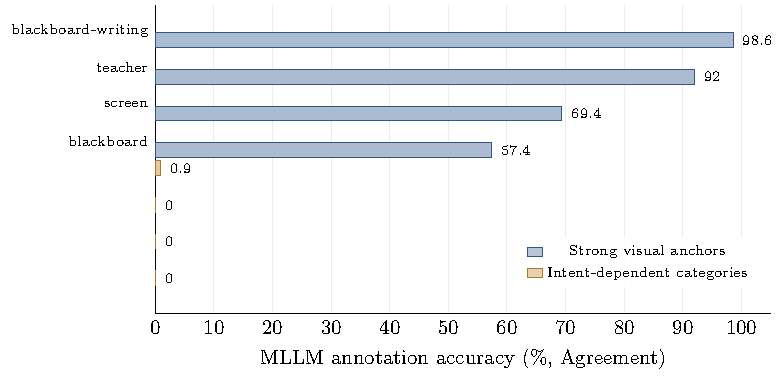
\includegraphics[width=0.92\linewidth]{fig_visual_anchoring_access.pdf}
\caption{Per-category MLLM annotation reliability on TeacherBehavior under
the Agreement strategy. Categories with explicit visual anchors are
annotated reliably, whereas categories requiring intent inference
drop to near-zero accuracy in the reported setting.}
\label{fig:visual_anchoring}
\end{figure}

Privacy-preserving representative crops in Fig~\ref{fig:visual_anchoring_examples}
make the same contrast concrete. Classes such as
\textit{blackboard-writing} and \textit{screen} are tied to localized
objects or surfaces that remain visually specific within one crop,
whereas \textit{answer} and \textit{guide} reduce to generic teaching
or teacher-student interaction postures despite carrying different
semantic labels.

\begin{figure}[!t]
\centering
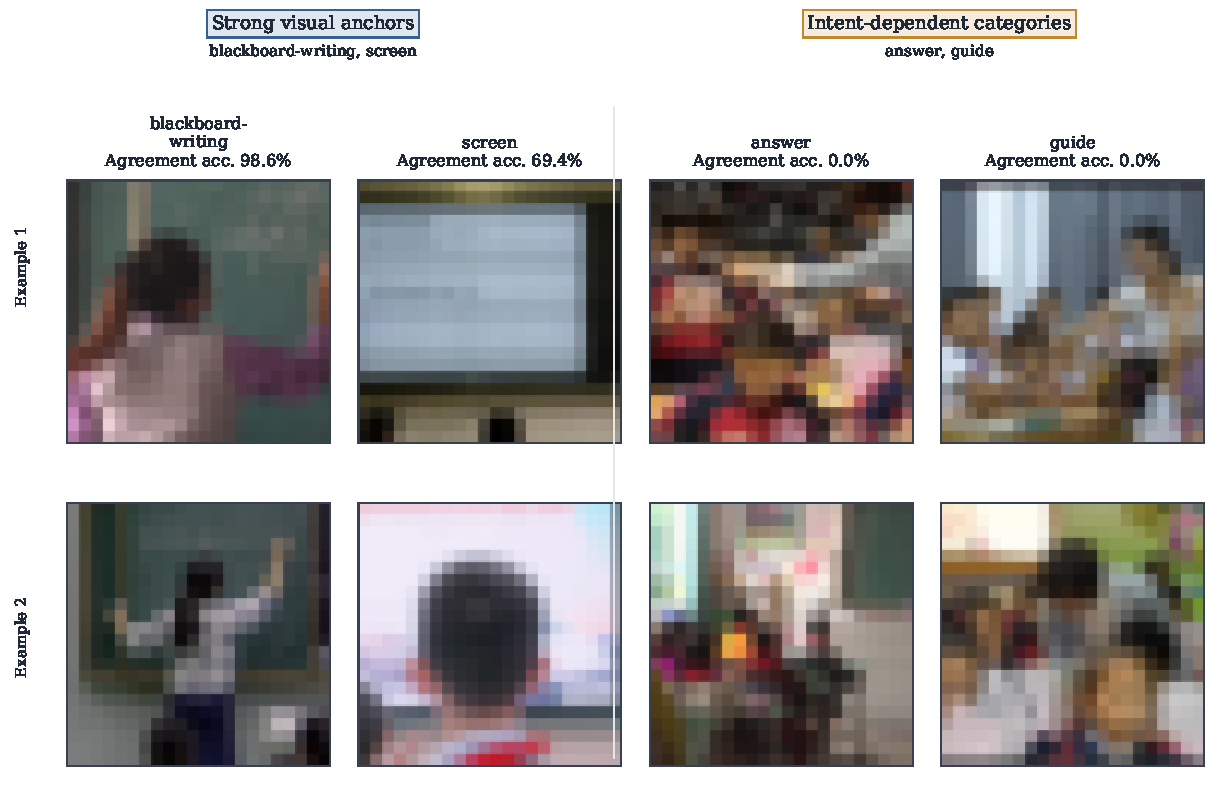
\includegraphics[width=0.98\linewidth]{fig_visual_anchoring_examples_access.pdf}
\caption{Privacy-preserving pixelated crops from the TeacherBehavior
validation agreement subset. High-anchor classes are associated with
localized visual cues, whereas low-anchor intent-defined classes remain
visually close to generic classroom interaction. The agreement
accuracies shown above each category match Table~\ref{tab:per_class}.}
\label{fig:visual_anchoring_examples}
\end{figure}

\subsection{Fine-Tuning Results}
\label{sec:finetune_results}

Table~\ref{tab:main_results} presents the complete $3 \times 3 \times 2$
result matrix together with the zero-shot CLIP baseline, while marking
which LoRA cells are targeted replications and which remain single-run
protocol-matched references.

\begin{table}[!t]
\caption{Validation accuracy (\%) of CLIP ViT-L/14 under all
experimental conditions. LP values report mean $\pm$ SD over repeated
seeds (all datasets: five seeds, 43--47); LoRA values report mean $\pm$ SD for the targeted five-seed
replication conditions (BowTurnHead and TeacherBehavior under None and
GT; seeds 43--47) and seed-42 protocol-matched references elsewhere.
\textbf{Bold} marks the best repeated-seed LP result per dataset;
single-run LoRA references marked with $^\dagger$ are not
included in best-result marking.
ZS = zero-shot CLIP baseline (no fine-tuning).
LP = linear probe. LoRA = low-rank adaptation.
These repeated-seed LoRA cells correspond only to those four
replicated conditions; see Finding~5 for the associated curve
analysis. The main conclusions about agreement filtering are drawn
primarily from repeated-seed LP results and annotation/retention
diagnostics; single-run LoRA cells are reported as protocol-matched
references.}
\label{tab:main_results}
\centering
\small
\resizebox{\columnwidth}{!}{%
\begin{tabular}{llcccccc}
\toprule
\multirow{2}{*}{\textbf{Dataset}} &
\multirow{2}{*}{\textbf{ZS}} &
\multicolumn{2}{c}{\textbf{None}} &
\multicolumn{2}{c}{\textbf{Agreement}} &
\multicolumn{2}{c}{\textbf{GT}} \\
\cmidrule(lr){3-4}\cmidrule(lr){5-6}\cmidrule(lr){7-8}
 & & LP & LoRA & LP & LoRA & LP & LoRA \\
\midrule
BowTurnHead
  & 42.37
  & 88.02$\pm$0.12 & 88.65$\pm$0.52
  & 15.53$\pm$1.00 & 19.69$^\dagger$
  & \textbf{93.35$\pm$0.08} & 97.91$\pm$0.10 \\
HandriseReadWrite
  & 56.88
  & 75.64$\pm$0.13 & 76.69$^\dagger$
  & 52.88$\pm$0.08 & 59.25$^\dagger$
  & \textbf{79.43$\pm$0.20} & 87.06$^\dagger$ \\
TeacherBehavior
  & 37.13
  & 42.38$\pm$0.07 & 43.22$\pm$0.46
  & 43.01$\pm$0.05 & 45.18$^\dagger$
  & \textbf{69.56$\pm$0.05} & 74.71$\pm$0.11 \\
\bottomrule
\end{tabular}
}
\end{table}

Table~\ref{tab:aux_baselines} reports two auxiliary training-strategy
baselines under the same CLIP ViT-L/14 feature protocol. Confidence
filtering approximately reproduces unfiltered pseudo-label LP
performance on BowTurnHead and HandriseReadWrite: 87.99\% versus
88.02\%, and 75.56\% versus 75.64\%, respectively. However, it produces
no usable TeacherBehavior training subset under the evaluated threshold
grid, indicating that CLIP-assigned confidence is uniformly low for the
Qwen pseudo-labels on this taxonomy; in practice, even the lowest
threshold in the grid retained no TeacherBehavior training crops. The
teacher--student baseline has a different task-dependent profile. It
slightly improves BowTurnHead, underperforms direct pseudo-label
supervision on HandriseReadWrite, and raises TeacherBehavior from
42.38\% under direct pseudo-label LP to 65.06\%, approaching the
69.56\% ground-truth LP reference. Because this teacher--student setting
uses a stratified 10\% labeled subset of the training split, it should be
read as a label-scarce semi-supervised reference, not as a label-free
pseudo-labeling baseline. Taken together, these baselines reinforce the
paper's conditional claim without identifying a uniformly dominant
training rule.

\begin{table}[!t]
\caption{Auxiliary filtering and teacher--student baselines under the
same CLIP ViT-L/14 feature protocol. Values report validation accuracy
(\%) over five seeds (43--47). Confidence filtering reports the best
nonempty threshold from the pre-specified grid
$\{0.3,0.5,0.6,0.7,0.8,0.9\}$; the value in parentheses gives the
selected threshold and mean training-set retention.}
\label{tab:aux_baselines}
\centering
\scriptsize
\resizebox{\columnwidth}{!}{%
\begin{tabular}{lccc}
\toprule
\textbf{Baseline} & \textbf{BowTurnHead} & \textbf{HandriseReadWrite} & \textbf{TeacherBehavior} \\
\midrule
Confidence filtering$^\ddagger$ & 87.99$\pm$0.22 ($\tau=0.3$; 100\%) & 75.56$\pm$0.24 ($\tau=0.3$; 100\%) & -- \\
Teacher--student & 89.17$\pm$1.06 & 68.08$\pm$0.23 & 65.06$\pm$0.36 \\
\bottomrule
\end{tabular}
}
\normalsize
\begin{minipage}{0.98\columnwidth}
\footnotesize
$^\ddagger$No TeacherBehavior confidence-filtering result is reported
because all evaluated thresholds, including $\tau=0.3$, retained zero
training samples.
\end{minipage}
\end{table}

Fig~\ref{fig:all_results_overview} visualizes the same result matrix
while keeping evidence levels explicit. The figure highlights
three trends that are less immediately visible from the table alone:
unfiltered pseudo-labels substantially improve over zero-shot on
BowTurnHead and HandriseReadWrite, agreement filtering is consistently
inferior to unfiltered pseudo-labels except for a marginal
TeacherBehavior LP gain of 0.63~pp, and ground-truth supervision
remains the upper reference across all datasets.

\begin{figure}[!t]
\centering

\includegraphics[width=0.98\linewidth]{fig_all_results_overview_access.pdf}
\caption{Overview of the full evaluation matrix. The plot includes the
three zero-shot baselines and all 18 CLIP fine-tuning conditions
formed by three datasets, three label sources, and two fine-tuning
methods. Solid bars denote repeated or replicated conditions; hatched
bars denote single-run references; error bars show $\pm 1$ SD when
available. ZS = zero-shot CLIP; LP = linear probing; LoRA = low-rank
adaptation; Agree = agreement-filtered pseudo-labels. Here, ZS bars
follow the baseline zero-shot setting used in Table~\ref{tab:main_results}
under the same bbox-crop validation protocol; LP bars use repeated-seed means,
whereas LoRA bars combine the targeted five-seed replication values
for BowTurnHead and TeacherBehavior under None and GT with
protocol-matched seed-42 references elsewhere.
Prompt-ensemble zero-shot values are reported separately in the
selective-analysis section.}
\label{fig:all_results_overview}
\end{figure}

\subsubsection{Cross-Model Robustness as a Boundary Check}

After the main downstream comparison, Tables~\ref{tab:crossmodel_overall}
and~\ref{tab:crossmodel_intent} summarise validation-set annotation accuracy
for the eleven tested MLLMs under the common bbox-crop and index-only prompting
protocol.
The purpose of this analysis is not to redefine the main pipeline, but
to test whether the category-level reliability pattern persists beyond
the original two-model pair, across model generations, architectures, and
parameter scales.

Three findings emerge from the expanded comparison.
First, no single annotator is uniformly best across datasets: Qwen3.5-35B-A3B
performs best on BowTurnHead (89.39\%), Qwen2 on HandriseReadWrite (70.59\%),
and Qwen3.5-27B on TeacherBehavior (52.19\%).
Second, a clear capability boundary exists on the \textit{guide} category:
earlier-generation models (Qwen2, Qwen2.5, LLaVA, Gemma3-27B) all score below
25\%, while newer-generation models (Qwen3.5-27B, Gemma4-31B) achieve 39--83\%,
showing that \textit{guide} is a model-capacity bottleneck rather than a
task-level impossibility.
Third, the \textit{answer} category remains below 23\% across all eleven models
(the best is Qwen3.6-35B-A3B at 22.4\%), consistent with a task-level
single-frame observability constraint that even the newest models cannot
overcome.

\begin{table}[!t]
\caption{Eleven-model cross-model robustness check of validation-set annotation
accuracy under a common bbox-crop and index-only prompting protocol.
Abbreviations: Q2.5-7B = Qwen2.5-VL-7B-Instruct;
Q2.5-32B = Qwen2.5-VL-32B-Instruct; G3-27B = Gemma-3-27B-IT;
Q3.5-27B = Qwen3.5-27B; Q3.5-35B = Qwen3.5-35B-A3B (MoE);
Q3.6-27B = Qwen3.6-27B; Q3.6-35B = Qwen3.6-35B-A3B (MoE, FP8);
G4-26B = Gemma4-26B-A4B-it (MoE); G4-31B = Gemma4-31B-it.
Qwen2 = Qwen2-VL-7B-Instruct; LLaVA = LLaVA-1.5-7B.
``---'' indicates the model was not evaluated on that dataset.
Values are bbox-level pseudo-label accuracy (\%). Best per dataset in bold.}
\label{tab:crossmodel_overall}
\centering
\scriptsize
\resizebox{\columnwidth}{!}{%
\begin{tabular}{lccccccccccc}
\toprule
\textbf{Dataset} & \textbf{Qwen2} & \textbf{LLaVA} & \textbf{Q2.5-7B} & \textbf{Q2.5-32B} & \textbf{G3-27B} & \textbf{Q3.5-27B} & \textbf{Q3.5-35B} & \textbf{Q3.6-27B} & \textbf{Q3.6-35B} & \textbf{G4-26B} & \textbf{G4-31B} \\
\midrule
BowTurnHead       & 82.55 & 14.76 & 84.86 & 63.78 & 75.19 & 84.93 & \textbf{89.39} & --- & 80.35 & 86.43 & 86.35 \\
HandriseReadWrite & \textbf{70.59} & 53.20 & 51.74 & 69.11 & 57.21 & --- & 62.71 & --- & 62.41 & 56.97 & 56.95 \\
TeacherBehavior   & 41.21 & 37.39 & 44.86 & 36.69 & 44.65 & \textbf{52.19} & 40.33 & 48.74 & 41.03 & 45.15 & 43.51 \\
\bottomrule
\end{tabular}
}
\normalsize
\end{table}

Table~\ref{tab:crossmodel_intent} reports per-category accuracy for
four key TeacherBehavior categories that illustrate the generational and
task-level boundaries.
The \textit{guide} category shows a clear generational divide: earlier-generation
models (Qwen2, Qwen2.5, LLaVA, Gemma3-27B) all score below 1\% except LLaVA
(24.05\%, likely a model-specific bias), while newer models reach
12.9--82.9\%, with Gemma4-31B achieving 82.9\%.
\textit{Answer} remains a near-universal failure: all eleven models score
below 23\%, with the best (Qwen3.6-35B-A3B at 22.4\%) still far below
usable annotation quality---consistent with a task-level single-frame
observability constraint.
\textit{Blackboard-writing} and \textit{screen} are reliably annotated
across all models (89.9--98.9\% and 48.1--88.8\%, respectively),
consistent with their strong visual signatures.
Qwen3.5-27B is the most balanced annotator on TeacherBehavior, with the
highest overall accuracy (52.19\%) and the best or near-best per-category
scores across all four classes shown.

\begin{table}[!t]
\caption{Eleven-model cross-model validation on four key TeacherBehavior
categories illustrating the generational boundary (\textit{guide}) and the
task-level constraint (\textit{answer}).
Values are validation-set bbox-level accuracy (\%).
$n$ = number of validation crops.}
\label{tab:crossmodel_intent}
\centering
\scriptsize
\resizebox{\columnwidth}{!}{%
\begin{tabular}{lccccccccccc}
\toprule
\textbf{Category} & \textbf{$n$} & \textbf{Qwen2} & \textbf{LLaVA} & \textbf{Q2.5-7B} & \textbf{Q2.5-32B} & \textbf{G3-27B} & \textbf{Q3.5-27B} & \textbf{Q3.5-35B} & \textbf{Q3.6-27B} & \textbf{Q3.6-35B} & \textbf{G4-26B} & \textbf{G4-31B} \\
\midrule
guide               & 449 & 0.22 & 24.05 & 0.00 & 0.89 & 0.22 & 52.34 & 24.50 & 39.20 & 12.92 & 36.04 & \textbf{82.85} \\
answer              & 853 & 0.00 & 0.00 & 1.17 & 5.16 & 1.41 & 17.70 & 18.87 & 8.56 & \textbf{22.39} & 0.35 & 9.38 \\
blackboard-writing  & 277 & 98.56 & 36.82 & 95.67 & --- & --- & 98.19 & 98.56 & \textbf{98.92} & 97.11 & 94.58 & 95.67 \\
screen              & 1959 & 69.37 & 13.78 & 56.41 & --- & --- & \textbf{88.82} & 73.51 & 74.27 & 68.86 & 52.78 & 48.09 \\
\bottomrule
\end{tabular}
}
\normalsize
\end{table}

%=================================================================
% 5. Discussion
%=================================================================
\subsubsection{Quality-Threshold Experiment with Qwen3.5-27B}

The cross-model validation identifies Qwen3.5-27B as the most balanced
annotator on TeacherBehavior (val-set accuracy 52.19\%, Table~\ref{tab:crossmodel_overall}),
substantially outperforming the original Qwen2-VL-7B annotator (41.21\%).
To test whether this 11pp improvement in annotation quality translates
into downstream fine-tuning gains, a targeted experiment was conducted
using Qwen3.5-27B pseudo-labels for CLIP fine-tuning on TeacherBehavior
under the same bbox-crop protocol, training settings, and seed
configuration as the main pipeline.
The Qwen3.5-27B training-set annotation accuracy is 50.3\% (the training
labels are used for fine-tuning; validation labels are only used for
quality measurement).

\begin{table}[!t]
\caption{TeacherBehavior fine-tuning results comparing Qwen2-VL-7B
pseudo-labels (annotation accuracy 41.2\%) and Qwen3.5-27B pseudo-labels
(annotation accuracy 50.3\%).
The zero-shot CAPE prompt-ensemble baseline is 53.43\%.
GT upper bounds: LP 69.56\%, LoRA 74.71\%.}
\label{tab:quality_threshold}
\centering
\begin{tabular}{lccc}
\toprule
\textbf{Training condition} & \textbf{Qwen2 (41.2\%)} & \textbf{Qwen3.5-27B (50.3\%)} & \textbf{$\Delta$} \\
\midrule
None + LP  & 42.38$\pm$0.07 & 55.29 & +12.91 \\
None + LoRA & 43.22$\pm$0.46 & 53.79 & +10.57 \\
Selective + LP & 58.37 & 62.10 & +3.73 \\
Selective + LoRA & --- & 53.20 & --- \\
\midrule
\emph{Zero-shot CAPE} & \emph{53.43} & \emph{53.43} & --- \\
\emph{GT + LP} & \emph{69.56$\pm$0.05} & \emph{---} & --- \\
\bottomrule
\end{tabular}
\end{table}

Figure~\ref{fig:quality_threshold} visualises the Qwen2 vs.\ Qwen3.5-27B
comparison for the three training conditions where both annotators have results.

\begin{figure}[!t]
\centering
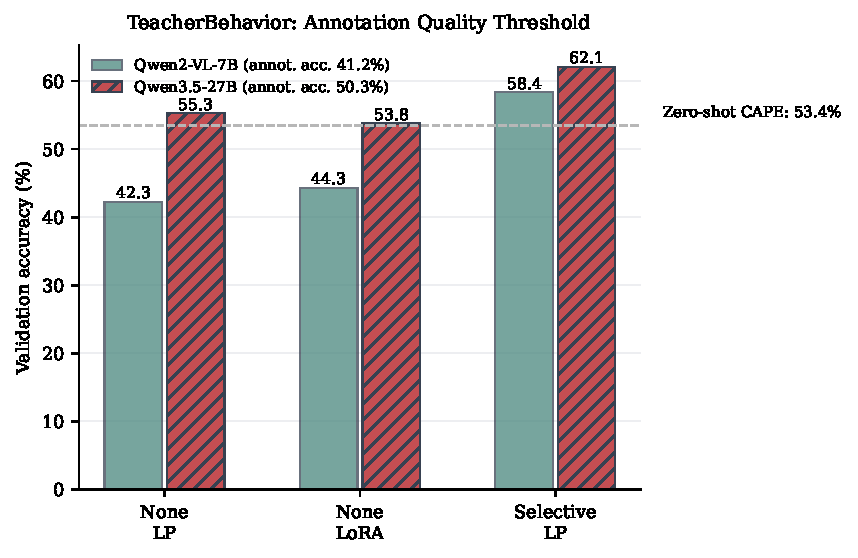
\includegraphics[width=0.85\linewidth]{fig_quality_threshold_access.pdf}
\caption{TeacherBehavior validation accuracy under Qwen2-VL-7B pseudo-labels
(annotation accuracy 41.2\%) versus Qwen3.5-27B pseudo-labels (50.3\%).
The dashed line marks the zero-shot CAPE prompt-ensemble baseline (53.43\%).
Qwen3.5-27B labels cross the zero-shot threshold for None+LP and Selective+LP,
while Qwen2-VL-7B labels remain below it for all conditions.}
\label{fig:quality_threshold}
\end{figure}

Three findings from this experiment are directly relevant to the paper's
central question.
First, the annotation quality threshold at which pseudo-label fine-tuning
begins to exceed the zero-shot baseline lies between 41\% and 50\%.
Qwen2-VL-7B labels (41.2\%) produce downstream accuracy below the
zero-shot baseline (None+LP: 42.38\% vs.\ 53.43\% zero-shot CAPE), while
Qwen3.5-27B labels (50.3\%) produce accuracy above it (None+LP: 55.29\%
vs.\ 53.43\% zero-shot CAPE).
This pinpoints a practical quality requirement for MLLM-assisted
annotation pipelines on TeacherBehavior-level task complexity.

Second, the selective-routing gain scales with annotator quality.
Under Qwen2-VL-7B pseudo-labels, selective+LP improves over None+LP
by 16.0pp (58.37\% vs.\ 42.38\%).
Under Qwen3.5-27B pseudo-labels, selective+LP reaches 62.10\%, an
improvement of 8.67pp over the zero-shot baseline compared with 4.94pp
for Qwen2-VL-7B.
This confirms that higher-quality base annotations amplify the benefit
of anchor-aware supervision routing, even with the same oracle router
(Scheme~B).

Third, LoRA remains unstable in the TeacherBehavior selective setting.
Selective+LoRA with Qwen3.5-27B labels achieves only 53.20\%---below
the zero-shot baseline and substantially below selective+LP (62.10\%).
This reinforces the earlier finding that LoRA is more vulnerable to
limited-data overfitting than linear probing when the training subset
is small (selective routing retains only high-anchor-class crops).

\section{Discussion}
\label{sec:discussion}

\subsection{Finding 1: Agreement Filtering Is Associated With
Data-Volume Loss, Distributional Bias, and Quality Ceiling}

The central lesson of Table~\ref{tab:annotation_quality},
Table~\ref{tab:main_results}, and Fig~\ref{fig:retention_curve} is not
simply that agreement filtering can underperform, but that the
diagnostics point to three interacting risks.
BowTurnHead is consistent with data-volume stress: the filter discards
enough examples to push training below a viable retention threshold.
HandriseReadWrite shows a different pattern: at moderate retention,
random subsampling remains close to the full-data baseline while the
agreement subset falls well below it, indicating that biased selection
may contribute beyond data reduction alone.
TeacherBehavior suggests a third regime: once pseudo-label noise becomes
the dominant bottleneck, increasing retention changes little, so
filtering does not meaningfully raise the attainable ceiling.

Fig~\ref{fig:distribution_shift} shows that the agreement subset does
not preserve the original training distribution. It over-selects
\textit{bow-head} in BowTurnHead (35.76\% to 63.40\%), shifts
HandriseReadWrite toward \textit{hand-raise} at the expense of
\textit{read} (30.52\% to 43.57\%; 50.80\% to 36.50\%), and in
TeacherBehavior over-selects \textit{teacher} while under-selecting
\textit{stand} (21.03\% to 26.45\%; 34.51\% to 31.32\%). The filter
changes not only data volume but also the class mix seen
during adaptation.

\begin{figure}[!t]
\centering

\includegraphics[width=0.98\linewidth]{fig_distribution_shift_access.pdf}
\caption{Class-composition shift between the full training split and
the agreement subset for each dataset. Labels on the agreement bars
report percentage-point change relative to the full training
distribution, making the direction and magnitude of selection bias
explicit.}
\label{fig:distribution_shift}
\end{figure}

These three regimes support a stronger practical warning than
``agreement is imperfect.''
Agreement is not a portable denoising rule in this setting because it
may simultaneously alter data volume, class composition, and sample
difficulty.
The five-seed LP averages remain the primary downstream evidence,
whereas the retention curves serve as mechanism checks.
Taken together, they imply that agreement-filtered subsets should be
treated as audited special cases, not as default pseudo-label training
data.
The cross-model comparison points in the same direction:
agreement quality varies materially with the model pair, so simple
annotator substitution does not turn the heuristic into a stable
strategy.

\subsection{Finding 2: Visual Anchoring Helps Diagnose When Agreement
Filtering Fails}

The most useful interpretation of Table~\ref{tab:per_class} is as a
diagnostic explanation for the failure patterns above.
Annotation reliability depends less on nominal model scale than on
whether a class is visually observable in a single crop.
Classes such as \textit{blackboard-writing} and \textit{teacher}
expose distinctive visual cues that MLLMs can align with pretraining
knowledge, whereas categories such as \textit{answer}, \textit{guide},
and \textit{on-stage interaction} depend more on pedagogical intent and
discourse context than on a unique frame-level signature.
The protocol-matched zero-shot CLIP results are used here as
an operational anchoring proxy, not as an independent causal
explanation: $\mathrm{AnchorProxy}(y)=\mathrm{Acc}^{\mathrm{ZS}}_{y}$
helps distinguish categories that are visually legible under the
current protocol from those that are not.

The eleven-model boundary check strengthens this interpretation.
Although the best annotator changes across datasets, the same
intent-dependent failure classes remain near-collapse under model
substitution.
That consistency suggests a task-level bottleneck, not a defect
specific to one annotator pair.
A complementary CMC check gives the same pattern in a CLIP-independent
form. Class-level CMC is strongly aligned with the zero-shot
AnchorProxy on HandriseReadWrite (Pearson $r=0.996$; Spearman
$\rho=0.500$) and moderately aligned on TeacherBehavior (Pearson
$r=0.573$; Spearman $\rho=0.439$). BowTurnHead has only two classes and
is reported descriptively, not as a correlation
analysis. These values do not make the proxy causal, but they reduce
the risk that the anchoring interpretation is merely an artefact of a
single CLIP zero-shot score.
In practical terms, the limiting issue is single-frame observability:
if the label cannot be recovered from an isolated crop, changing the
annotator is unlikely to solve the problem.
Under this reading, visual anchoring is best treated as a screening
diagnostic for when pseudo-label supervision is plausible.
High-anchor categories are plausible candidates for pseudo-label
supervision, whereas low-anchor categories should default to stronger
prompting, added audit, human annotation, or richer temporal and
multimodal evidence.

More broadly, these findings challenge a common assumption in
pseudo-label pipelines: that inter-model agreement is a reliable proxy
for label quality. In this setting, agreement preferentially
retains samples on which both models express the same perceptual bias,
instead of samples that are objectively easier to classify. When two
annotators inherit similar pretraining corpora or architectural
inductive biases, their agreement can reflect shared blind spots instead
of genuine label confidence. Under that view,
agreement filtering is better understood not as a denoising
operation, but as a selection mechanism whose behaviour depends on the
model pair and on the visual discriminability of the target
categories.

\begin{figure}[!t]
\centering
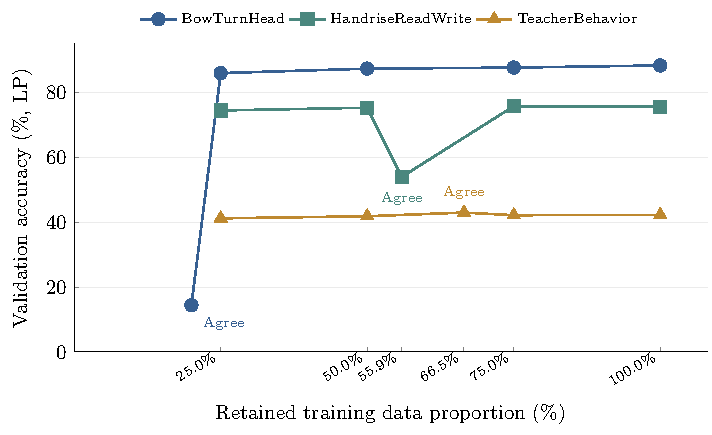
\includegraphics[width=0.94\linewidth]{fig_retention_curve_access.pdf}
\caption{Retention-ratio curves for BowTurnHead, HandriseReadWrite,
and TeacherBehavior under linear probing with unfiltered pseudo-labels
(None strategy), augmented with the agreement-filtered endpoint
(labelled ``Agree''). All plotted points are fixed-seed diagnostic
runs (seed 42), whereas Table~\ref{tab:main_results} reports
repeated-seed LP means for the main downstream comparison.
The x-axis reports \emph{training-set} retention rates, whereas
Table~\ref{tab:annotation_quality} reports \emph{validation-set}
retention rates for annotation quality. Random subsampling remains
stable above the critical retention threshold for all three datasets.
The agreement-selected endpoint falls far below the random-retention
trend for BowTurnHead and HandriseReadWrite, whereas TeacherBehavior
shows only a small positive deviation.}
\label{fig:retention_curve}
\end{figure}

\subsection{Finding 3: Annotation Quality Thresholds and the Selective-Routing Upper Bound}

Two related findings constrain when pseudo-label supervision is likely to
be useful.
First, the quality-threshold experiment (Table~\ref{tab:quality_threshold})
identifies the annotation accuracy range at which pseudo-label fine-tuning
crosses the zero-shot baseline.
Qwen2-VL-7B labels at 41.2\% annotation accuracy produce downstream
accuracy below zero-shot (42.38\% vs.\ 53.43\% CAPE), while Qwen3.5-27B
labels at 50.3\% annotation accuracy surpass the baseline (55.29\% vs.\
53.43\%).
The critical threshold for TeacherBehavior-level task complexity therefore
lies between 41\% and 50\%, providing a practical quality target for
MLLM-assisted annotation pipelines.

Second, the selective-routing diagnostic (Table~\ref{tab:selective_results})
shows that its benefit scales with base annotation quality.
Selective+LP improves over zero-shot by 4.94pp with Qwen2 labels and by
8.67pp with Qwen3.5-27B labels (62.10\% vs.\ 53.43\%).
This supports the interpretation that anchor-aware supervision routing
amplifies, rather than replaces, the benefit of higher-quality annotations.
The result remains a boundary diagnostic, not a deployable method, because
Scheme~B uses oracle routing and the AnchorProxy is coupled to the
zero-shot branch.

\subsection{Finding 4: Task Complexity Moderates the Benefit of
Pseudo-Label Fine-Tuning}

The downstream comparison answers the central question
conditionally.
Unfiltered pseudo-labels can beat zero-shot CLIP when the task is
visually grounded enough that label noise does not erase the training
signal.
That is the pattern on BowTurnHead and, more moderately, on
HandriseReadWrite.
The same strategy is far less persuasive on TeacherBehavior, where the
label semantics depend more heavily on intent and interaction context.

Ground-truth fine-tuning clarifies the distinction.
Clean labels remain strongly useful across all three datasets, so the
weak pseudo-label result on TeacherBehavior should not be read as
evidence that the task itself is resistant to adaptation.
It is instead evidence that task complexity and label semantics jointly
determine whether pseudo-label supervision is worth using.
The auxiliary baselines sharpen this point. Confidence filtering
recovers the unfiltered LP regime on BowTurnHead and HandriseReadWrite
but fails to retain any TeacherBehavior samples under the evaluated
thresholds, consistent with uniformly weak CLIP confidence on that
taxonomy. Conversely, the train-split teacher--student baseline raises
TeacherBehavior to 65.06\%, close to the 69.56\% GT LP reference, while
falling to 68.08\% on HandriseReadWrite. The useful conclusion is
not that self-training is universally better, but that
TeacherBehavior's weak direct pseudo-label result is primarily a label
quality problem under this protocol.
A practical decision rule follows: pseudo-label fine-tuning is most
plausible when classes are visually grounded and semantically stable;
as intent dependence increases, selective human annotation becomes more
valuable.

\subsection{Finding 5: The Attainable Performance Ceiling Is More
Strongly Locked by Label Quality Than by Optimisation Path}

The five-seed LoRA replications sharpen the same conclusion from a
different angle.
What changes most across conditions is not only mean accuracy but the
ceiling itself.
Ground-truth supervision produces both higher validation scores and
much lower cross-seed variance, whereas pseudo-label supervision keeps
the model in a noisier regime.
Across the replicated BowTurnHead and TeacherBehavior settings, the
mean cross-seed SD is 0.107\% under GT supervision versus 0.495\%
under pseudo-label supervision.
On TeacherBehavior in particular, the pseudo-label setting can fit the
training set almost perfectly while validation remains trapped in a
narrow band.
That pattern is more consistent with memorising inconsistent decision
boundaries than with simply choosing the wrong checkpoint or
optimisation schedule.

This matters because it limits one easy counterargument to the main
results.
The weak pseudo-label outcome cannot be explained away by saying that
LoRA merely needed more careful tuning.
Under this single-frame protocol, optimisation changes the
training trajectory more than it changes the attainable validation
regime.
The remaining single-run LoRA cells should still be read cautiously,
but the replicated seeds are sufficient to support a narrower
conclusion: label quality constrains both performance and stability
more strongly than optimisation path in the settings where the paper
makes its strongest claims.

\subsection{TeacherBehavior Case Study: What the Selective-Routing
Gain Does and Does Not Show}

The TeacherBehavior case study makes the boundary condition concrete.
When agreement-based selection is unreliable, category-aware routing
can still be informative as an upper-bound diagnostic, even though the
present Scheme~B implementation is not directly deployable.
Table~\ref{tab:selective_results} summarises the result.

\begin{table}[!t]
\caption{Comparison of annotation strategies on TeacherBehavior
(validation accuracy, \%). The selective strategy uses pseudo-labels
for high-anchor classes and zero-shot CLIP for low-anchor classes.
High-anchor: blackboard-writing, teacher, screen, blackboard.
Low-anchor: guide, answer, on-stage interaction, stand.
The zero-shot baseline in this table uses the prompt-ensemble setting.
\textbf{Selective routing uses ground-truth category as oracle routing
variable at evaluation time and represents a diagnostic upper bound,
not a deployable pipeline or a deployable-method comparison.}}
\label{tab:selective_results}
\centering
\resizebox{\columnwidth}{!}{%
\begin{tabular}{lccc}
\toprule
\textbf{Strategy} & \textbf{Overall (8-cls)} &
\textbf{High-anchor (4-cls)} & \textbf{Low-anchor (4-cls)} \\
\midrule
Zero-shot CLIP (prompt ensemble) & 53.43 & --- & --- \\
None + LP (full pseudo) & 42.38 & --- & --- \\
Oracle selective + LP & 58.37 & 72.74 & 38.44 \\
GT + LP (upper bound) & 69.56 & --- & --- \\
\bottomrule
\end{tabular}
}
\end{table}

The gain comes from the high-anchor portion of the taxonomy, while the
low-anchor classes remain better handled by the zero-shot branch.
That is precisely why the result should not be interpreted as a new
universal pipeline.
It depends on oracle routing and on a fine-tuning setup that preserves
the zero-shot branch.

This constraint also explains why LoRA is a poor fit for Scheme~B.
Once the shared encoder is altered, the fallback branch for low-anchor
categories is no longer stable.
The case study is most useful as a design implication.
If a taxonomy mixes visually explicit and intent-dependent classes,
selective routing may be worth exploring, but only with an explicit
routing mechanism and without presenting the oracle result as
deployment-ready.

\subsection{Limitations}
\label{sec:limitations}

Several limitations should be noted.
First, the main annotation pipeline evaluates two 7B-scale locally
deployable MLLMs, and the expanded cross-model robustness analysis spans
eleven models across seven families: Qwen2-VL-7B, LLaVA-1.5-7B,
Qwen2.5-VL-7B-Instruct, Qwen2.5-VL-32B-Instruct, Qwen3.5-27B,
Qwen3.5-35B-A3B, Qwen3.6-27B, Qwen3.6-35B-A3B, Gemma-3-27B-IT,
Gemma4-26B-A4B-it, and Gemma4-31B-it.
This broader evidence reduces concern that the reported failure
patterns are unique to one particular model pair, but broader
validation across more datasets, prompt regimes, and multimodal model
families remains necessary.
Whether larger-scale or video-aware models materially improve
annotation reliability for intent-dependent categories remains an open
question.
Second, the annotation pipeline uses image-level prompts without
chain-of-thought reasoning or few-shot examples; more sophisticated
prompting strategies may improve accuracy on intent-dependent
categories. In particular, the index-only output constraint used here
standardises parsing but does not expose uncertainty, so prompt
sensitivity and abstention-aware prompting remain open questions.
Third, the study uses a single benchmark
(SCB) from Chinese K--12 classrooms; generalisability to other
educational contexts and cultural settings requires further
investigation.
Fourth, the selective annotation experiment evaluates only linear
probing; LoRA is incompatible with Scheme~B due to encoder-level
interference with the zero-shot classifier, and alternative
architectures that decouple the fine-tuned head from the shared
encoder (e.g., adapter layers, separate encoder branches) are left
for future work.
Fifth, the main LP conditions are averaged over five random seeds
(all datasets: five seeds, 43--47), but the
LoRA replication now covers BowTurnHead and TeacherBehavior under None
and GT across five seeds (43--47). However, the remaining LoRA
settings and several diagnostic analyses remain single-run
protocol-matched evaluations. The reported differences
should still be interpreted as controlled diagnostic
comparisons rather than as full estimates of training variance across
all conditions.
The study does not support formal significance claims for
small differences in conditions that remain single-run, and future
work should extend repeated-seed evaluation to the remaining LoRA and
auxiliary diagnostic analyses, together with bootstrap- or
permutation-based uncertainty estimates.
The eleven-model robustness analysis and the Qwen3.5-27B quality-threshold
experiment partly strengthen external validity with respect to annotator
choice, but they do not remove the internal validity limitations in the
downstream fine-tuning matrix.
The fine-tuning hyper-parameters are also held fixed across the main
comparisons, so systematic learning-rate sensitivity is not evaluated
in this study.
Sixth, the paper treats visual anchoring as a
diagnostic concept that is operationalised here with a task-specific
proxy ($\mathrm{AnchorProxy}(y)=\mathrm{Acc}^{\mathrm{ZS}}_{y}$), rather
than a universal quantitative variable.
Because this proxy is itself derived from classifier performance, it
should be interpreted as an operational diagnostic, not a
standalone explanatory construct.
The CMC analysis adds a CLIP-independent consistency check, but it is
still descriptive and does not establish a causal measurement of
anchoring.
Future work should evaluate more general category-level indicators and
test whether their association with pseudo-label accuracy is stable
across datasets and model families.
Seventh, the practical training-time baselines included here remain
deliberately narrow. Confidence filtering uses a CLIP-assisted
probability proxy because the index-only MLLM annotation protocol does
not expose calibrated model uncertainty, and the teacher--student
baseline uses one linear-probe self-training design with a stratified
10\% labeled subset of the training split.
Prompt-adaptation methods such as CoOp/CoCoOp, calibrated MLLM
abstention, and more elaborate semi-supervised objectives remain
outside this comparison.
Eighth, although the retention-ratio analysis and distribution-shift
metrics (total-variation distance, KL divergence) provide partial
controls for data-volume and sampling-bias effects, the three failure
mechanisms identified for agreement filtering---data-volume collapse,
distributional bias, and quality ceiling---are not fully causally
isolated in the current experimental design. Agreement-filtered
subsets differ from random subsets simultaneously in data volume,
class distribution, sample difficulty, and visual diversity, so the
present mechanism attribution should be read as diagnostically
motivated, not causally verified. Controlled experiments that
independently vary these factors---for example, class-balanced
resampling matched to the agreement subset distribution, or
difficulty-stratified retention curves---are left for future work.

\subsection{Reproducibility Statement}
\label{sec:repro}

The repository implements these analysis modules using the following
scripts at the repository root:
zero-shot evaluation (baseline and prompt-ensemble settings,
\path{step0b_cape_zeroshot.py}),
MLLM annotation (\path{step1_llm_annotate.py} and
\path{cross_model_annotate.py}),
filtering analysis (\path{step2_filter_analysis.py}),
CLIP fine-tuning (\path{step3_clip_finetune.py}),
selective annotation (\path{step4_selective_annotation.py}),
retention-ratio curve (\path{step5_retention_curve.py}), and
repeated-seed aggregation (\path{summarize_repeated_seeds.py}).
The auxiliary strategy and consistency analyses are implemented in
\path{confidence_filtering.py},
\path{teacher_student_self_training.py}, and
\path{cross_model_consistency.py}.
The submitted artifact includes \path{environment.yml} and
\path{requirements.txt} for environment reconstruction. The experiment
snapshot used for manuscript preparation is identified by repository
commit \texttt{e21ae3d09c8d1577eeb75d1a29e2661cf757e877}; the archived
artifact should preserve the exact submitted snapshot together with the
generated result files.
LP main-matrix results are averaged over repeated seeds (all
datasets: five seeds, 43--47); targeted LoRA replications for BowTurnHead and
TeacherBehavior under None and GT use seeds 43--47, while remaining
LoRA and selected diagnostics are single-seed/fixed-seed evaluations
(seed 42).
Table-level provenance is as follows: annotation-quality and confusion
tables are generated by the filtering-analysis module, the main
fine-tuning matrix by the CLIP fine-tuning and repeated-seed summary
modules, the selective-routing table by the selective-annotation
module, the auxiliary-baseline table by the confidence-filtering and
teacher--student modules, and the retention-ratio figure by the
retention-curve module.
The SCB dataset is publicly available~\cite{scb_dataset}.
The code repository and run configurations used for the analysis are
publicly available at \url{https://github.com/zhanglizhuo/llm-annotation}
(accessed on 27 April 2026), including the pipeline scripts, archived
shell entry points, and result directories referenced in this paper.
For reproducibility review, the repository should remain publicly
accessible and preserve per-module run recipes for the main tables and
figures.

%=================================================================
% 6. Conclusions
%=================================================================
\section{Conclusions}
\label{sec:conclusions}

The paper asked a practical question: when can MLLM-generated
pseudo-labels improve classroom behavior recognition, and when does
agreement filtering make them worse instead of better?
Within the SCB benchmark, the answer is conditional rather
than global.
Pseudo-labels help when the target classes are visually anchored
enough that single-frame crops preserve the evidence needed for
labeling.
They do not help reliably when the taxonomy is dominated by
intent-dependent classes, and cross-model agreement is not a safe
remedy because it may remove training volume, distort class
composition, and preserve shared bias instead of correctness.

The evidence supporting that answer is consistent across the
manuscript.
Category-level annotation results show a sharp divide between visually
anchored classes and intent-dependent classes.
The repeated-seed LP matrix shows that unfiltered pseudo-labels can
outperform zero-shot CLIP on visually grounded datasets, whereas the
clearest counterexample appears on BowTurnHead, where Agreement+LP
falls to 15.53\% $\pm$ 1.00\% while None+LP reaches 88.02\%
$\pm$ 0.12\%.
The targeted LoRA replications indicate that label quality constrains
not only attainable accuracy but also run-to-run stability.
The quality-threshold experiment locates the critical annotation accuracy
range at which pseudo-label fine-tuning crosses the zero-shot baseline on
TeacherBehavior (between 41\% and 50\%), and the expanded eleven-model
cross-model validation reveals a generational boundary on
\textit{guide} while confirming that \textit{answer} remains below 23\%
across all tested models.
The CMC diagnostic, the auxiliary confidence-filtering and
teacher--student baselines, the oracle Scheme~B diagnostic, and the
eleven-model robustness check then bound the claim: pseudo-label
supervision is most plausible for high-anchor categories, not as a
universal replacement for human annotation or temporal and multimodal
evidence.

The practical implication is not ``filter harder'' but
``screen the task first.''
For SCB-like single-frame classroom sensing, a conservative workflow is
to audit category anchoring before committing annotation budget,
avoid agreement filtering as a default denoising rule,
select an annotator with task-level accuracy above the zero-shot
threshold (approximately 50\% for TeacherBehavior-level complexity),
use pseudo-label supervision mainly on high-anchor categories,
and reserve low-anchor categories for stronger zero-shot prompts,
temporal or multimodal sensing, or human labelling.
Under this interpretation, the contribution of the paper is a
reproducible reliability-audit protocol for deciding when MLLM
pseudo-labeling is useful in classroom behavior recognition, together
with diagnostic evidence on the main failure modes that make it
unreliable in this setting.

\section*{Author Contributions}
Conceptualization, Y.M. and L.Z.; methodology, Y.M. and L.Z.; software,
L.Z.; validation, Y.M. and L.Z.; formal analysis, Y.M.; investigation,
Y.M.; data curation, Y.M. and L.Z.; visualization, L.Z.; writing---original
draft preparation, Y.M.; writing---review and editing, Y.M. and L.Z.;
supervision, L.Z.

\section*{Conflicts of Interest}
The authors declare no conflicts of interest.

\section*{Data and Code Availability}
The three SCB sub-datasets used in this study, plus the excluded
single-class Discuss set, are publicly available on Hugging Face at
\url{https://huggingface.co/datasets/wintonYF/SCB-Dataset} (accessed on
27 April 2026). These datasets are externally released resources and are
not owned by this study. The experiment code and archived run
configurations are available at
\url{https://github.com/zhanglizhuo/llm-annotation} (accessed on 27 April 2026).
The repository was publicly accessible at the time of access.

\section*{Acknowledgment}
The authors thank wintonYF and all contributors who created and maintained
the public SCB dataset releases used in this study.

\begin{thebibliography}{99}

\bibitem{brophy2000teaching}
Brophy J. Teaching. Brussels (Belgium): International Academy of
Education; 2000.

\bibitem{anderson2004classroom}
Anderson LW. Increasing Teacher Effectiveness. 2nd ed. Paris
(France): UNESCO; 2004.

\bibitem{zhang2020classroom_cnn}
Zhang L, Zhu Z.
Automatic classroom observation: Student behavior recognition using
deep learning. IEEE Access. 2020;8:149079-149088.

\bibitem{bai2023qwen}
Bai J, Bai S, Yang S, Wang S, Tan S, Wang P, et al.
Qwen-VL: A versatile vision-language model for understanding, localization,
text reading, and beyond. arXiv [Preprint]. 2023 [cited 2026 Apr 27].
Available from: https://arxiv.org/abs/2308.12966

\bibitem{liu2023llava}
Liu H, Li C, Wu Q, Lee YJ.
Visual instruction tuning.
In: Advances in Neural Information Processing Systems (NeurIPS);
2023; New Orleans, LA, USA. Vol. 36.

\bibitem{gilardi2023chatgpt}
Gilardi F, Alizadeh M, Kubli M.
ChatGPT outperforms crowd workers for text-annotation tasks.
Proc Natl Acad Sci U S A. 2023;120:e2305016120.

\bibitem{he2023annollm}
He X, Lin Z, Gong Y, Jin A, Zhang H, Lin C, et al.
AnnoLLM: Making large language models to be better crowdsourced annotators.
arXiv [Preprint]. 2023 [cited 2026 Apr 27]. Available from:
https://arxiv.org/abs/2303.16854

\bibitem{cao2025latteclip}
Cao M, Bontempelli A, Tonioni A, Tombari F, Solin A, Kannala J, et al.
LatteCLIP: Unsupervised CLIP fine-tuning via LMM-synthetic texts.
In: Proceedings of the IEEE/CVF Winter Conference on Applications of
Computer Vision (WACV); 2025; Tucson, AZ, USA.

\bibitem{li2022classroom_transformer}
Li Z, Li B, Li X.
A survey of video-based classroom behavior analysis.
Appl Sci. 2022;12:10428.

\bibitem{whitehill2014automated}
Whitehill J, Serpell Z, Lin YC, Foster A, Movellan JR.
The faces of engagement: Automatic recognition of student
engagement from facial expressions.
IEEE Trans Affect Comput. 2014;5:86-98.

\bibitem{donnelly2017automatic}
Donnelly PJ, Blanchard N, Samei B, Olney AM, Sun X, Ward B, et al.
Automatic prediction of presentation quality with behavior image
sequences.
In: Proceedings of the ACM International Conference on Multimodal
Interaction (ICMI); 2017; Glasgow, Scotland, UK. pp. 369-377.

\bibitem{dillenbourg2011classroom}
Dillenbourg P, Zufferey G, Alavi H, Jermann P, Do-Lenh S, Bonnard Q,
et al.
Classroom orchestration: The third circle of usability.
In: Proceedings of the International Conference on
Computer-Supported Collaborative Learning (CSCL); 2011; Hong Kong,
China. pp. 510-517.

\bibitem{radford2021learning}
Radford A, Kim JW, Hallacy C, Ramesh A, Goh G, Agarwal S, et al.
Learning transferable visual models from natural language supervision.
In: Proceedings of the International Conference on Machine Learning
(ICML); 2021; Virtual Event. pp. 8748-8763.

\bibitem{schuhmann2022laion5b}
Schuhmann C, Beaumont R, Vencu R, Gordon C, Wightman R, Cherti M,
et al. LAION-5B: An open large-scale dataset for training next
generation image-text models. In: Advances in Neural Information
Processing Systems (NeurIPS); 2022; New Orleans, LA, USA. Vol. 35.

\bibitem{cherti2023reproducible}
Cherti M, Beaumont R, Wightman R, Wortsman M, Ilharco G, Gordon C,
et al.
Reproducible scaling laws for contrastive language-image learning.
In: Proceedings of the IEEE/CVF Conference on Computer Vision and
Pattern Recognition (CVPR); 2023; Vancouver, BC, Canada.
pp. 22084-22095.

\bibitem{zhai2023sigmoid}
Zhai X, Mustafa B, Kolesnikov A, Beyer L.
Sigmoid loss for language image pre-training.
In: Proceedings of the IEEE/CVF International Conference on Computer
Vision (ICCV); 2023; Paris, France. pp. 11975-11986.

\bibitem{sun2023eva02}
Sun Q, Fang Y, Wu L, Wang X, Cao Y.
EVA-02: A visual representation powerhouse for dense prediction tasks.
arXiv [Preprint]. 2023 [cited 2026 Apr 27]. Available from:
https://arxiv.org/abs/2303.11331

\bibitem{fang2023data}
Fang A, Jose AM, Jain A, Schmidt L, Toshev A, Shankar V.
Data filtering networks.
arXiv [Preprint]. 2023 [cited 2026 Apr 27]. Available from:
https://arxiv.org/abs/2309.17425

\bibitem{wang2022medclip}
Wang Z, Wu Z, Agarwal D, Sun J.
MedCLIP: Contrastive learning from unpaired medical images and text.
In: Proceedings of the Conference on Empirical Methods in Natural
Language Processing (EMNLP); 2022; Abu Dhabi, UAE. pp. 3876-3887.

\bibitem{liu2024remoteclip}
Liu F, Chen D, Guan Z, Zhou X, Zhu J, Zhou J.
RemoteCLIP: A vision language foundation model for remote sensing.
IEEE Trans Geosci Remote Sens. 2024;62:1-16.

\bibitem{wang2021actionclip}
Wang M, Xing J, Liu Y.
ActionCLIP: A new paradigm for video action recognition.
arXiv [Preprint]. 2021 [cited 2026 Apr 27]. Available from:
https://arxiv.org/abs/2109.08472

\bibitem{zhou2022learning}
Zhou K, Yang J, Loy CC, Liu Z.
Learning to prompt for vision-language models.
Int J Comput Vis. 2022;130:2337-2348.

\bibitem{zhou2022conditional}
Zhou K, Yang J, Loy CC, Liu Z.
Conditional prompt learning for vision-language models.
In: Proceedings of the IEEE/CVF Conference on Computer Vision and
Pattern Recognition (CVPR); 2022; New Orleans, LA, USA.
pp. 16816-16825.

\bibitem{zhang2024zero}
Zhang Y, Rao Y, Liu M.
Zero-shot facial expression recognition with multimodal large language
models. arXiv [Preprint]. 2024 [cited 2026 Apr 27]. Available from:
https://arxiv.org/abs/2401.12508

\bibitem{liu2024llavanext}
Liu H, Li C, Wu Q, Lee YJ.
LLaVA-NeXT: Improved reasoning, OCR, and world knowledge in
vision-language chat models. arXiv [Preprint]. 2024 [cited 2026 May 7].
Available from: https://arxiv.org/abs/2401.00368

\bibitem{qwen2025technical}
Qwen Team.
Qwen2.5-VL technical report. arXiv [Preprint]. 2025 [cited 2026 May 7].
Available from: https://arxiv.org/abs/2502.13923

\bibitem{chen2024internvl2}
Chen Z, Wang K, Cao Y, Yu J, Zhou W, Li H, et al.
InternVL2: Better than the best at every scale.
arXiv [Preprint]. 2024 [cited 2026 May 7]. Available from:
https://arxiv.org/abs/2412.05271

\bibitem{yue2024mmmu}
Yue X, Ni Y, Zhang K, Zheng T, Liu Y, Huang W, et al.
MMMU: A massive multi-discipline multimodal understanding and
reasoning benchmark for expert AGI. In: Proceedings of the IEEE/CVF
Conference on Computer Vision and Pattern Recognition (CVPR); 2024;
Seattle, WA, USA. pp. 9551-9561.

\bibitem{sohn2020fixmatch}
Sohn K, Berthelot D, Carlini N, Zhang Z, Zhang H, Raffel CA, et al.
FixMatch: Simplifying semi-supervised learning with consistency
and confidence.
In: Advances in Neural Information Processing Systems (NeurIPS);
2020; Virtual Event. Vol. 33. pp. 596-608.

\bibitem{zhang2021flexmatch}
Zhang B, Wang Y, Hou W, Wu H, Wang J, Okumura M, et al.
FlexMatch: Boosting semi-supervised learning with curriculum pseudo
labeling.
In: Advances in Neural Information Processing Systems (NeurIPS);
2021; Virtual Event. Vol. 34. pp. 18408-18419.

\bibitem{laine2016temporal}
Laine S, Aila T.
Temporal ensembling for semi-supervised learning.
arXiv [Preprint]. 2016 [cited 2026 Apr 27]. Available from:
https://arxiv.org/abs/1610.02242

\bibitem{snow2008cheap}
Snow R, O'Connor B, Jurafsky D, Ng AY.
Cheap and fast---but is it good? Evaluating non-expert annotations
for natural language tasks.
In: Proceedings of the Conference on Empirical Methods in Natural
Language Processing (EMNLP); 2008; Honolulu, HI, USA. pp. 254-263.

\bibitem{scb_dataset}
SCB Dataset [Internet]. Available from:
https://huggingface.co/datasets/wintonYF/SCB-Dataset [cited 2026 Apr 1].

\bibitem{hu2022lora}
Hu EJ, Shen Y, Wallis P, Allen-Zhu Z, Li Y, Wang S, et al.
LoRA: Low-rank adaptation of large language models.
In: Proceedings of the International Conference on Learning
Representations (ICLR); 2022; Virtual Event.

\end{thebibliography}

\EOD

\end{document}